\documentclass[12pt, a4paper]{article}

%\documentclass{article}
\usepackage{graphicx} % Required for inserting images
\usepackage{geometry}
\usepackage[style=numeric, sorting=none]{biblatex}
\usepackage{amsmath}
\usepackage{amsfonts}
\usepackage{amssymb}

\addbibresource{refs.bib}



\title 
{Multivariate and Velocity-Resolved Reverberation in NGC~5548:\\
Astrophysical Motivation for an Information-Based Analysis of Continuum--BLR Coupling}
\author{ Ayan Mitra, Vasilios Zarikas}
\date{June 2026}





\begin{document}

\maketitle

%\begin{document}


\begin{abstract}
Reverberation mapping has become one of the most powerful tools for probing the unresolved inner structure of active galactic nuclei. In its classical form, the method relates continuum variability to delayed emission-line responses and thereby constrains the characteristic scale of the broad-line region, the black-hole mass, and the geometry and kinematics of the line-emitting gas. However, modern high-cadence campaigns have shown that the astrophysical situation is richer than the traditional single-driver, single-response picture suggests. In well-observed systems such as NGC~5548, continuum interband delays, velocity-resolved H$\beta$ reverberation, and episodes of anomalous line--continuum decorrelation indicate that the observed optical or ultraviolet continuum is not always an adequate representation of the ionizing field seen by the broad-line region. These results motivate a more explicitly multivariate and velocity-resolved analysis of reverberation data, especially under conservative time-domain conditions that minimize artificial structure introduced by incomplete temporal overlap. In this paper we focus on the astrophysical problem: how the optical continuum and the blue wing, core, and red wing of H$\beta$ jointly encode the dynamical response of the low-ionization broad-line region in NGC~5548. The information-decomposition formalism employed later in the paper is not introduced here; instead, this Introduction develops the astrophysical background, motivates the scientific questions, and places the present work in the context of the reverberation-mapping literature.
\end{abstract}








\section{Introduction}

Active galactic nuclei (AGN) are powered by accretion onto supermassive black holes and radiate over a broad range of wavelengths through a compact but highly structured central engine. The standard observational picture includes an accretion disk that produces much of the optical and ultraviolet continuum, a hot corona responsible for the X-ray emission, a broad-line region (BLR) composed of dense photoionized gas moving at velocities of order \(10^3\) to \(10^4\) km s\(^{-1}\), and more distant dusty material that reprocesses the radiation field at infrared wavelengths \cite{Peterson2004,Netzer2013,Cackett2021}. Because these regions are too compact to resolve directly in most AGN, temporal variability provides one of the few effective ways to infer their sizes, structure, and coupling.

Reverberation mapping exploits the fact that fluctuations in the central ionizing source are echoed by delayed responses in remote reprocessing or emission-line regions. In its simplest linearized form, the response of an emission line \(L(t)\) to a driving continuum \(C(t)\) may be written as
\begin{equation}
L(t) = \int \Psi(\tau)\,C(t-\tau)\,d\tau,
\end{equation}
where \(\Psi(\tau)\) is the transfer function or delay distribution. The classical use of this formalism has been to derive a characteristic lag \(\tau\), associate it with a BLR radius \(R \sim c\tau\), and combine that scale with the line width to estimate the black-hole mass under a virial assumption \cite{Peterson2004,BentzKatz2015}. This framework has been extremely successful and remains foundational to AGN black-hole mass scaling relations.

Nevertheless, the astrophysical interpretation of reverberation data has become progressively more subtle. The quantity that drives the broad emission lines is the ionizing continuum, particularly in the extreme ultraviolet and soft X-ray bands, whereas the continuum actually monitored in many optical reverberation campaigns is a more accessible proxy, often the flux near \(5100\) \AA. As a result, the measured lag between an observed continuum band and an emission line need not correspond to a direct causal connection between those two observables alone. Instead, both may be responding, with different delays and different filtering, to a latent radiation field that is only imperfectly traced by the observed bands \cite{Cackett2021}. The question is therefore not merely what the lag is, but whether the monitored continuum contains the relevant information needed to explain the line response.

This issue is underscored by continuum reverberation mapping. A series of high-cadence monitoring programs has revealed that ultraviolet and optical continuum bands in AGN are delayed with respect to one another, with delays that often grow systematically with wavelength as expected for a thermally stratified accretion disk. However, the measured lags are frequently larger than predicted by the simplest geometrically thin, optically thick accretion-disk models \cite{Fausnaugh2016,Fausnaugh2017,Edelson2019,Cackett2021}. These results suggest that the observed continuum variability is not fully described by a minimal reprocessing picture and may involve additional processes such as intrinsic accretion-rate fluctuations, diffuse continuum emission, complex irradiation geometry, or nontrivial radiative transfer. From the standpoint of BLR reverberation, this implies that optical continuum light curves may not be interpreted as pristine drivers without further caution.

NGC~5548 is the canonical source in which these concerns become impossible to ignore. It is one of the most intensively monitored Seyfert galaxies and has served as a cornerstone of reverberation mapping for decades. It has played a major role in calibrating broad-line lags, virial mass estimates, and radius--luminosity relations, while more recent campaigns have transformed it into a benchmark for multiwavelength and velocity-resolved reverberation analysis \cite{Peterson2002,BentzKatz2015,Cackett2021}. In particular, the AGN STORM campaign delivered one of the richest reverberation datasets ever obtained, including optical and ultraviolet continuum monitoring, extensive spectroscopy, and detailed velocity-delay information for several broad lines \cite{DeRosa2015,Pei2017,Horne2021}.

These observations revealed that NGC~5548 is not well described by a stationary one-zone BLR driven by a single observed continuum proxy. Velocity-resolved reverberation results showed clear structure across the H$\beta$ profile, with the line wings and core participating differently in the reverberation pattern \cite{Pei2017,Horne2021}. The interpretation of these data points toward a BLR that is radially stratified and kinematically complex, possibly including multiple components or zones rather than a single homogeneous distribution of clouds \cite{Horne2021,LongDexter2025}. This immediately motivates a shift away from purely integrated-line analyses. If the blue wing, line core, and red wing carry different dynamical information, then treating H$\beta$ as a single scalar time series necessarily compresses part of the astrophysical content of the data.

An even more striking complication emerged during the same source's monitoring history: the so-called ``holiday'' in NGC~5548. During part of the AGN STORM campaign, the broad emission lines became partially decorrelated from the observed UV continuum, even though they had previously tracked it closely. The leading interpretation is that an obscuring wind or shielding structure modified the ionizing spectral energy distribution reaching the BLR while leaving the observed UV continuum comparatively unaffected \cite{Dehghanian2019}. The importance of this result cannot be overstated. It demonstrates directly that an observed continuum channel may cease to be a faithful tracer of the radiation field relevant for BLR photoionization. Consequently, a line--continuum lag analysis may look physically incomplete not because the line has stopped reverberating, but because the monitored continuum is no longer the appropriate driver proxy.

This broader lesson is now reinforced by work across the reverberation-mapping literature. Velocity-resolved H$\beta$ studies increasingly show that BLR kinematics are diverse across AGN and may evolve over time, with some sources displaying signatures consistent with inflow, others with outflow, and others with virialized or mixed dynamics \cite{Du2018,Wang2025,Feng2024}. In parallel, changing-look AGN have demonstrated that the relation between continuum state and broad-line emission can undergo dramatic reorganization on humanly accessible timescales \cite{RicciTrakhtenbrot2023}. Although changing-look phenomena are not the focus of the present study, they help establish a wider astrophysical principle: the mapping between observed continuum, ionizing continuum, and line-emitting gas is not guaranteed to be stationary.

Within this context, NGC~5548 is particularly well suited for a more conservative, multivariate analysis of the reverberation problem. The source offers high-quality continuum monitoring, extensive H$\beta$ spectroscopy, and a rich legacy of prior reverberation results against which new analyses may be compared. At the same time, it is sufficiently complex to require such an approach. If one asks only for an integrated H$\beta$ lag relative to the optical continuum, much of the internal structure of the reverberation process is averaged away. By contrast, if one treats the blue wing, core, and red wing of H$\beta$ as distinct observables, new astrophysical questions become accessible. Does the core behave primarily as an echo of the continuum, or does it also depend on information already present in the wings? Are the two wings symmetric in their predictive role, as one might expect in an idealized virialized BLR, or does one side of the profile carry systematically different dynamical information? Can the observed optical continuum alone account for the velocity-resolved response, or do hidden drivers and internal line-component couplings remain necessary?

These questions are not purely methodological. They arise naturally from long-standing astrophysical uncertainties about the BLR and the continuum source. The BLR is expected to be sensitive to the ionizing continuum, but in practice the ionizing continuum is usually unobserved. The optical continuum is measurable but is itself part of a reverberating accretion-flow system and may therefore contain both intrinsic and reprocessed variability components \cite{Fausnaugh2017,Cackett2021}. The H$\beta$ line is observable with high fidelity, but its integrated flux merges together multiple kinematic regions whose relative responses may differ. Once velocity-resolved spectroscopy is available, the astrophysical challenge becomes one of causal disentanglement among observables that are neither independent nor trivially ordered in a simple driver--response chain.

A number of established approaches address parts of this challenge. Interpolated cross-correlation methods and related lag estimators remain the standard tools for continuum--line reverberation analysis and continue to provide essential baseline measurements \cite{Peterson2004,WhitePeterson1994}. JAVELIN and related stochastic-process approaches model reverberation as a damped random walk continuum filtered by a transfer function, thereby improving lag estimation and uncertainty quantification in many cases \cite{Zu2011,Zu2013}. Velocity-delay mapping and dynamical modeling aim to reconstruct the geometry and kinematics of the BLR directly from the line-profile response \cite{Pancoast2014,Horne2021}. Continuum reverberation studies focus on interband disk lags and the thermal structure of the accretion flow \cite{Fausnaugh2016,Fausnaugh2017,Edelson2019}. Each of these approaches has been productive, but they are typically tailored to a specific projection of the problem: pairwise lags, transfer-function fitting, dynamical inversion, or continuum size scaling.

What remains comparatively underexplored is the specific astrophysical question of how multiple simultaneously observed channels jointly constrain the future evolution of one chosen component of the system, especially when those channels include both the continuum and velocity-resolved line segments. In other words, once the H$\beta$ profile has been decomposed into blue wing, core, and red wing light curves, and once a conservative common time interval is imposed, the natural problem is no longer simply ``what is the lag?'' It becomes: how much of the future behavior of one velocity component is already encoded in the continuum, how much is encoded in another part of the line profile, and how much lies beyond the information available in the monitored observables? That is the astrophysical problem motivating the present paper.

The emphasis on strict temporal overlap is also not incidental. Irregular cadence, seasonal gaps, and unequal overlap among observed channels are intrinsic features of AGN monitoring data. Any multivariate time-series analysis is therefore vulnerable to spurious structure introduced by aggressive interpolation, extrapolation across gaps, or implicit assumptions about the simultaneity of channels that were not truly observed together. In the context of NGC~5548, where the scientific questions depend sensitively on comparing the optical continuum to distinct H$\beta$ velocity components, it is essential to work under conservative overlap conditions. The goal is not to maximize sample size at all costs, but to preserve physical interpretability. A shorter but genuinely shared time interval is preferable to a longer one in which apparent multivariate structure may be partly synthetic.

The present paper is therefore built around a deliberately astrophysical motivation. We seek to determine how the optical continuum near \(5100\) \AA\ and the velocity-resolved components of H$\beta$ in NGC~5548 are coupled when the data are restricted to robust common overlap. Our interest is not merely in recovering a known lag, but in characterizing the continuum--BLR system as a multichannel, time-dependent structure. We focus on the blue wing, line core, and red wing because these components are directly linked to the low-ionization BLR geometry and kinematics, and because they allow one to ask whether different parts of the line profile participate differently in the reverberation process. This is the astrophysical motivation for the analysis developed in the sections that follow.

The methodological framework used later in the paper is based on information decomposition, but we intentionally postpone its formal description. The present Introduction has a different role: to show why such an analysis is astrophysically warranted. The literature has already established that NGC~5548 exhibits continuum interband lags, velocity-resolved H$\beta$ structure, partial line--continuum decoupling during the holiday, and evidence for a multicomponent BLR. The natural next step is not simply to add another lag estimator, but to investigate the reverberation data in a way that is explicitly multivariate, velocity-resolved, and conservative with respect to temporal overlap. That is the problem we address here.

The structure of this paper is as follows. In Section~2 we describe the observations, spectral processing, and the construction of strictly overlapping continuum and velocity-resolved H$\beta$ time series. In Section~3 we introduce the formal information-based framework used to quantify the coupling among the observables. In Section~4 we present the main results for continuum--line and line--line relationships, including robustness tests and comparisons with classical reverberation measures. In Section~5 we discuss the implications for the structure of the BLR in NGC~5548, the role of hidden or imperfectly observed drivers, and the interpretation of multivariate reverberation signals. Section~6 summarizes our conclusions and outlines possible extensions to larger AGN samples and to other broad emission lines.


\section{Synergistic--Unique--Redundant Decomposition (SURD) for Time Series}
\label{sec:surd_method}

\subsection{Problem formulation}

Consider a collection of \(N\) observed stochastic processes,
\begin{equation}
\mathbf{Q}(t)=\bigl(Q_1(t),Q_2(t),\ldots,Q_N(t)\bigr),
\end{equation}
sampled at discrete times \(t=t_n\). For a chosen target index \(j\), the goal is to quantify how much information about the future state
\begin{equation}
Q_j^+ \equiv Q_j(t+\Delta T)
\end{equation}
is contained in the observed variables at time \(t\) and, crucially, to decompose that predictive information into \emph{redundant}, \emph{unique}, and \emph{synergistic} contributions \cite{MartinezSanchez2024SURD}.

The central motivation is that in multivariate systems, pairwise predictive measures such as Granger causality or transfer entropy can establish that a variable is informative about a target, but they do not in general distinguish whether that information is:
\begin{enumerate}
    \item unique to one predictor,
    \item duplicated across several predictors, or
    \item available only from a joint observation of several predictors.
\end{enumerate}
SURD is designed precisely to perform that decomposition in a time-series setting \cite{MartinezSanchez2024SURD,Schreiber2000,WilliamsBeer2010}.

\subsection{Information-theoretic preliminaries}

Let \(Y\equiv Q_j^+\) denote the target and let \(\mathbf{X}\) denote the vector of observed predictors. For discrete variables, the Shannon entropy is
\begin{equation}
H(Y)=-\sum_{y} p(y)\log_2 p(y),
\end{equation}
and the conditional entropy of \(Y\) given \(\mathbf{X}\) is
\begin{equation}
H(Y\mid \mathbf{X})=-\sum_{y,\mathbf{x}} p(y,\mathbf{x})\log_2 p(y\mid \mathbf{x}).
\end{equation}
The mutual information between \(Y\) and \(\mathbf{X}\) is
\begin{equation}
I(Y;\mathbf{X})=H(Y)-H(Y\mid \mathbf{X})
=\sum_{y,\mathbf{x}} p(y,\mathbf{x})
\log_2\frac{p(y,\mathbf{x})}{p(y)p(\mathbf{x})}.
\label{eq:mi_total}
\end{equation}
This quantity measures the total predictive information about the future target that is available in the observed present state \cite{Shannon1948,CoverThomas2006}.

In SURD, the unexplained part of the future is interpreted as a \emph{causality leak},
\begin{equation}
\Delta I_{\mathrm{leak}\to j}=H(Y\mid \mathbf{X}),
\label{eq:leak_def}
\end{equation}
so that the forward information balance reads
\begin{equation}
H(Y)=I(Y;\mathbf{X})+\Delta I_{\mathrm{leak}\to j}.
\label{eq:forward_balance}
\end{equation}

Equation \eqref{eq:forward_balance} is one of the core ideas of SURD: the future uncertainty of the target splits into an observed part, explained by the measured variables, and an unobserved part, attributed to hidden or unmeasured influences \cite{MartinezSanchez2024SURD}.

\subsection{From total predictive information to causal components}

Let the predictor vector be
\begin{equation}
\mathbf{X} = (X_1,\ldots,X_M),
\end{equation}
where the \(X_\alpha\) may correspond either to different physical variables at the same time, or to different lagged copies of the same variables. SURD decomposes the observable predictive information \(I(Y;\mathbf{X})\) into additive components:
\begin{equation}
I(Y;\mathbf{X})
=
\sum_{\mathcal{A}\in\mathcal{C}} \Delta I_{\mathcal{A}\to j}^{R}
+
\sum_{\alpha=1}^{M} \Delta I_{\alpha\to j}^{U}
+
\sum_{\mathcal{A}\in\mathcal{C}} \Delta I_{\mathcal{A}\to j}^{S},
\label{eq:surd_master}
\end{equation}
where:
\begin{itemize}
    \item \(\Delta I_{\mathcal{A}\to j}^{R}\) is the \emph{redundant} contribution from the group of predictors indexed by \(\mathcal{A}\),
    \item \(\Delta I_{\alpha\to j}^{U}\) is the \emph{unique} contribution of predictor \(X_\alpha\),
    \item \(\Delta I_{\mathcal{A}\to j}^{S}\) is the \emph{synergistic} contribution from the group \(\mathcal{A}\),
    \item \(\mathcal{C}\) denotes all non-singleton subsets of \(\{1,\dots,M\}\).
\end{itemize}
The full future entropy therefore obeys
\begin{equation}
H(Y)=
\sum_{\mathcal{A}\in\mathcal{C}} \Delta I_{\mathcal{A}\to j}^{R}
+
\sum_{\alpha=1}^{M} \Delta I_{\alpha\to j}^{U}
+
\sum_{\mathcal{A}\in\mathcal{C}} \Delta I_{\mathcal{A}\to j}^{S}
+
\Delta I_{\mathrm{leak}\to j}.
\label{eq:full_surd_balance}
\end{equation}

The three causal types have the following interpretation \cite{MartinezSanchez2024SURD}:
\begin{itemize}
\item{Redundant:}  
the same predictive information is shared across several predictors,\\
\item{Unique:}  
a predictor contains information not available from any other predictor alone,\\
\item {Synergistic:}  
information appears only when several predictors are observed jointly.
\end{itemize}

\subsection{Specific mutual information and statewise decomposition}

A key feature of SURD is that the source of predictability may depend on which \emph{particular future event} \(y\) occurs. To resolve this dependence, SURD works first at the level of \emph{specific mutual information} \cite{DeWeeseMeister1999,Butts2003,MartinezSanchez2024SURD}.

For a particular target state \(Y=y\), the specific mutual information between \(y\) and a predictor set \(\mathbf{X}_{\mathcal{A}}\) is
\begin{equation}
\tilde{\imath}_{\mathcal{A}}(y)
\equiv
\tilde{\imath}\bigl(y;\mathbf{X}_{\mathcal{A}}\bigr)
=
\sum_{\mathbf{x}_{\mathcal{A}}}
\frac{p(y,\mathbf{x}_{\mathcal{A}})}{p(y)}
\log_2
\frac{p(y,\mathbf{x}_{\mathcal{A}})}{p(y)\,p(\mathbf{x}_{\mathcal{A}})}.
\label{eq:specific_mi}
\end{equation}
The ordinary mutual information is recovered by averaging over target states:
\begin{equation}
I\bigl(Y;\mathbf{X}_{\mathcal{A}}\bigr)
=
\sum_{y} p(y)\,\tilde{\imath}_{\mathcal{A}}(y).
\label{eq:mi_from_specific}
\end{equation}

The conceptual reason for introducing \(\tilde{\imath}_{\mathcal{A}}(y)\) is that different predictors may be informative for different target outcomes. A predictor may, for example, strongly constrain large positive target excursions while another may mainly constrain negative or low-amplitude states. A decomposition performed only at the level of the average mutual information can obscure this state dependence. SURD therefore computes the information contributions for each \(y\), decomposes them into redundant, unique, and synergistic increments, and only afterwards averages over \(y\) \cite{MartinezSanchez2024SURD}.

\subsection{Statewise incremental construction of SURD}

Let \(\mathfrak{P}^\ast(\{1,\dots,M\})\) denote the set of all non-empty subsets of predictors. For each subset \(\mathcal{A}\in \mathfrak{P}^\ast(\{1,\dots,M\})\), one computes
\begin{equation}
\tilde{\imath}_{\mathcal{A}}(y)
=
\tilde{\imath}\bigl(y;\mathbf{X}_{\mathcal{A}}\bigr).
\end{equation}
SURD then considers the collection of all these values for a fixed target state \(y\) and identifies the \emph{increments} in predictive information that arise as one moves from smaller to larger subsets of predictors \cite{MartinezSanchez2024SURD}. Denoting these statewise increments schematically by
\begin{equation}
\Delta \tilde{\imath}_{\mathcal{A}}(y),
\end{equation}
the classification rule is:
\begin{itemize}
    \item an increment assigned to one predictor alone contributes to \(\Delta \tilde{\imath}_{\alpha}^{U}(y)\),
    \item an increment shared across several predictors contributes to \(\Delta \tilde{\imath}_{\mathcal{A}}^{R}(y)\),
    \item an increment that arises only when a collection of predictors is observed jointly contributes to \(\Delta \tilde{\imath}_{\mathcal{A}}^{S}(y)\).
\end{itemize}

The averaged causal components are then
\begin{align}
\Delta I_{\mathcal{A}\to j}^{R}
&=
\sum_{y} p(y)\,\Delta \tilde{\imath}_{\mathcal{A}}^{R}(y),\\
\Delta I_{\alpha\to j}^{U}
&=
\sum_{y} p(y)\,\Delta \tilde{\imath}_{\alpha}^{U}(y),\\
\Delta I_{\mathcal{A}\to j}^{S}
&=
\sum_{y} p(y)\,\Delta \tilde{\imath}_{\mathcal{A}}^{S}(y).
\end{align}
This construction ensures that the total observable predictive information is recovered exactly:
\begin{equation}
I(Y;\mathbf{X})
=
\sum_{\mathcal{A}\in\mathcal{C}} \Delta I_{\mathcal{A}\to j}^{R}
+
\sum_{\alpha=1}^{M} \Delta I_{\alpha\to j}^{U}
+
\sum_{\mathcal{A}\in\mathcal{C}} \Delta I_{\mathcal{A}\to j}^{S}.
\label{eq:observable_recovery}
\end{equation}

\subsection{Two-source case}

For two predictors \(X_1\) and \(X_2\), the decomposition reduces to
\begin{equation}
I(Y;X_1,X_2)
=
\Delta I_{12\to j}^{R}
+
\Delta I_{1\to j}^{U}
+
\Delta I_{2\to j}^{U}
+
\Delta I_{12\to j}^{S}.
\label{eq:two_source_total}
\end{equation}
Consistency with the single-predictor mutual informations requires
\begin{align}
I(Y;X_1) &= \Delta I_{12\to j}^{R} + \Delta I_{1\to j}^{U},\\
I(Y;X_2) &= \Delta I_{12\to j}^{R} + \Delta I_{2\to j}^{U}.
\end{align}
Hence the synergistic contribution may be written as the remainder
\begin{equation}
\Delta I_{12\to j}^{S}
=
I(Y;X_1,X_2)
-
\Delta I_{12\to j}^{R}
-
\Delta I_{1\to j}^{U}
-
\Delta I_{2\to j}^{U}.
\end{equation}
This form makes the interpretation transparent: the synergy is the part of the joint predictive information that cannot be accounted for by the redundant and unique terms.

\subsection{Extension to time series with multiple lags}

For time-series applications, the predictor vector is typically augmented with lagged copies of the observed variables. If one includes \(p\) past lags per variable, the predictor vector becomes
\begin{equation}
\mathbf{X}(t)=
\Bigl[
Q_1(t),Q_1(t-\Delta T_1),\ldots,Q_1(t-\Delta T_p),\;
Q_2(t),Q_2(t-\Delta T_1),\ldots,Q_N(t-\Delta T_p)
\Bigr].
\label{eq:lagged_vector_general}
\end{equation}
For example, with \(N=2\) variables and one additional lag,
\begin{equation}
\mathbf{X}(t)=
\bigl[
Q_1(t),Q_1(t-\Delta T),Q_2(t),Q_2(t-\Delta T)
\bigr].
\label{eq:lagged_vector_two}
\end{equation}
SURD then treats each lagged component as one predictor channel and applies the same decomposition machinery to the enlarged predictor set \cite{MartinezSanchez2024SURD}. In this way, the method can distinguish:
\begin{itemize}
    \item self-causation from \(Q_j(t-\Delta T_k)\) to \(Q_j(t+\Delta T)\),
    \item cross-causation from \(Q_i(t-\Delta T_k)\) to \(Q_j(t+\Delta T)\),
    \item redundancy between different lags,
    \item synergy between variables and lags.
\end{itemize}

This is particularly important when several lagged channels may encode overlapping predictive content. For example, adding \(Q_j(t)\) and \(Q_j(t-\Delta T)\) can increase redundancy rather than revealing new independent causal pathways. SURD is expressly designed to make that distinction \cite{MartinezSanchez2024SURD}.

\subsection{Contemporaneous and mixed lagged dependencies}

A further advantage of the formalism is that the predictor vector can include variables at time \(t+\Delta T\) other than the target itself, thereby allowing the analysis of contemporaneous or effectively sub-resolution interactions \cite{MartinezSanchez2024SURD}. In practice, one excludes the target variable from the contemporaneous predictor set to avoid trivial self-determination, but permits other variables measured on the same time slice. Thus, a generic predictor vector may mix present, lagged, and contemporaneous channels:
\begin{equation}
\mathbf{X}(t)=
\bigl[
\text{past lags},
\text{present variables},
\text{contemporaneous non-target variables}
\bigr].
\end{equation}
The same decomposition \eqref{eq:full_surd_balance} then applies.

\subsection{Normalization and interpretation}

Because the observable predictive information is conserved by construction, the unique, redundant, and synergistic terms are naturally normalized by the total observable mutual information:
\begin{equation}
\widehat{\Delta I}_{\mathcal{A}\to j}^{R}
=
\frac{\Delta I_{\mathcal{A}\to j}^{R}}{I(Y;\mathbf{X})},
\qquad
\widehat{\Delta I}_{\alpha\to j}^{U}
=
\frac{\Delta I_{\alpha\to j}^{U}}{I(Y;\mathbf{X})},
\qquad
\widehat{\Delta I}_{\mathcal{A}\to j}^{S}
=
\frac{\Delta I_{\mathcal{A}\to j}^{S}}{I(Y;\mathbf{X})}.
\label{eq:normalized_atoms}
\end{equation}
These normalized terms sum to unity:
\begin{equation}
\sum_{\mathcal{A}\in\mathcal{C}}\widehat{\Delta I}_{\mathcal{A}\to j}^{R}
+
\sum_{\alpha=1}^{M}\widehat{\Delta I}_{\alpha\to j}^{U}
+
\sum_{\mathcal{A}\in\mathcal{C}}\widehat{\Delta I}_{\mathcal{A}\to j}^{S}
=1.
\end{equation}
The leak is normalized instead by the total entropy of the target:
\begin{equation}
\widehat{\Delta I}_{\mathrm{leak}\to j}
=
\frac{\Delta I_{\mathrm{leak}\to j}}{H(Y)}
=
\frac{H(Y\mid\mathbf{X})}{H(Y)}.
\label{eq:normalized_leak}
\end{equation}
Hence:
\begin{itemize}
    \item \(\widehat{\Delta I}_{\mathrm{leak}\to j}\approx 0\) means the observed predictors account for almost all predictive information about the target,
    \item \(\widehat{\Delta I}_{\mathrm{leak}\to j}\approx 1\) means most of the target's future uncertainty remains unexplained by the observed variables.
\end{itemize}

\subsection{Practical estimation}

In applications, the probabilities appearing in Eqs.~\eqref{eq:mi_total} and \eqref{eq:specific_mi} must be estimated from finite data. The original SURD work uses histogram-based and transport-map-based estimators depending on dimensionality and sample size \cite{MartinezSanchez2024SURD}. In a histogram implementation, one discretizes the predictor-target space into bins and estimates
\begin{equation}
p(y,\mathbf{x}) \approx \frac{n(y,\mathbf{x})}{N_{\mathrm{samples}}},
\end{equation}
where \(n(y,\mathbf{x})\) is the bin count. The resulting empirical joint distribution is then used to compute all required marginal and conditional probabilities. More sophisticated estimators, such as transport maps, are advantageous in high dimensions because the number of bins required by direct histograms grows exponentially with the number of predictors.

Algorithmically, the SURD workflow for a target \(Q_j^+\) is:
\begin{enumerate}
    \item choose the predictor vector \(\mathbf{X}\), including variables, lags, or contemporaneous channels;
    \item estimate the probability distributions \(p(y,\mathbf{x}_{\mathcal{A}})\) for all relevant predictor subsets \(\mathcal{A}\);
    \item compute the specific informations \(\tilde{\imath}_{\mathcal{A}}(y)\) for every target state \(y\);
    \item decompose the statewise increments into redundant, unique, and synergistic parts;
    \item average over \(y\) to obtain \(\Delta I^R\), \(\Delta I^U\), and \(\Delta I^S\);
    \item compute the leak from Eq.~\eqref{eq:leak_def};
    \item normalize the observable components by \(I(Y;\mathbf{X})\) and the leak by \(H(Y)\).
\end{enumerate}

\subsection{Properties and assumptions}

SURD has several properties that are important in time-series applications \cite{MartinezSanchez2024SURD}:
\begin{enumerate}
    \item \textbf{Non-negativity:} all redundant, unique, synergistic, and leak terms are non-negative.
    \item \textbf{Additivity:} the observable predictive information is exactly partitioned into \(R\), \(U\), and \(S\) terms.
    \item \textbf{Sensitivity to nonlinear dependence:} because the construction is based on mutual information, it is not restricted to linear couplings.
    \item \textbf{Compatibility with lagged and contemporaneous predictors:} time-lag structure enters through the predictor vector.
    \item \textbf{Hidden-variable diagnostics:} the leak quantifies the fraction of future uncertainty left unexplained by the observed variables.
\end{enumerate}

The main assumptions are those common to observational information-theoretic causality analysis:
\begin{itemize}
    \item the processes are sufficiently stationary over the analysis interval for probability estimation to be meaningful,
    \item the chosen time resolution is physically relevant,
    \item the sample size is adequate for the selected probability estimator,
    \item and causal interpretation remains limited to the observed variables plus the quantified unresolved contribution represented by the leak.
\end{itemize}

\subsection{Summary}

SURD starts from the predictive information \(I(Q_j^+;\mathbf{X})\) between a future target and a multivariate predictor state. It then decomposes that predictive information into state-averaged unique, redundant, and synergistic contributions, while retaining the conditional entropy \(H(Q_j^+\mid \mathbf{X})\) as an explicit measure of hidden or unobserved influence. Its time-series extension is straightforward: past lags, present variables, and even contemporaneous non-target channels are simply incorporated into the predictor vector. For multivariate dynamical systems, this yields a decomposition that is richer than pairwise lag measures because it distinguishes direct predictive effects from duplicated information and from genuinely joint multivariate effects \cite{MartinezSanchez2024SURD,WilliamsBeer2010}.

\section{Observations, Spectral Processing, and Strict Overlap Alignment}
\label{sec:data_processing}

To evaluate the capabilities of the SURD algorithm on real-world astrophysical data, we analyze the well-monitored Seyfert 1 galaxy NGC~5548. This source has a rich legacy of reverberation mapping, including the high-cadence AGN STORM campaign \cite{DeRosa2015,Pei2017}. Our analysis utilizes two main datasets: the optical continuum flux at 5100~\AA\ and velocity-resolved H\(\beta\) emission line profiles.

\subsection{Data Products and MJD Correction}

The 5100~\AA\ continuum light curve is obtained from the AGN Watch databases (specifically, \texttt{c5100.dat}), spanning a long duration of several years. The integrated H\(\beta\) emission line light curve is similarly taken from clean AGN Watch compilations (\texttt{ngc5548\_agnwatch\_hb\_clean.csv}).

The velocity-resolved spectroscopy files, containing H\(\beta\) profiles, were processed from individual \texttt{.spc} files. The filenames (following the template \texttt{nXXXXXma.spc}) contain an embedded time indicator where the numerical part \texttt{XXXXX} represents a Julian Date (JD) offset. Specifically, we confirmed the filename-to-MJD conversion:
\begin{equation}
\mathrm{MJD} = \mathrm{XXXXX} - 10000.
\end{equation}
Applying this correction aligns the spectroscopic observations from the filename values in the range 57512--59255 to the physical Modified Julian Date (MJD) range of 47512--49255, matching the historical campaigns of the late 1980s and early 1990s.

We extract three kinematic components from the H\(\beta\) profile:
\begin{enumerate}
    \item \textbf{Blue Wing:} integrated flux in the velocity range \([-3000, -1000]\)~\(\mathrm{km\,s^{-1}}\).
    \item \textbf{Line Core:} integrated flux in the velocity range \([-1000, +1000]\)~\(\mathrm{km\,s^{-1}}\).
    \item \textbf{Red Wing:} integrated flux in the velocity range \([+1000, +3000]\)~\(\mathrm{km\,s^{-1}}\).
\end{enumerate}
A summary of the raw data products is presented in Table~\ref{tab:data_properties}.

\begin{table}[ht]
\centering
\begin{tabular}{lccccc}
\hline
\textbf{Data Product} & \textbf{Points} & \textbf{MJD Min} & \textbf{MJD Max} & \textbf{Median Cadence} & \textbf{Source File} \\
\hline
5100~\AA\ Continuum & 1548 & 47509.00 & 52264.62 & 1.00 days & \texttt{c5100.dat} \\
Integrated H\(\beta\) & 1248 & 47509.00 & 52174.23 & 1.05 days & AGN Watch \\
H\(\beta\) Blue Wing & 247 & 47512.00 & 49255.00 & 5.00 days & \texttt{hb\_profiles\_extracted} \\
H\(\beta\) Line Core & 247 & 47512.00 & 49255.00 & 5.00 days & \texttt{hb\_profiles\_extracted} \\
H\(\beta\) Red Wing & 247 & 47512.00 & 49255.00 & 5.00 days & \texttt{hb\_profiles\_extracted} \\
\hline
\end{tabular}
\caption{Properties of the optical continuum and velocity-resolved H\(\beta\) light curves for NGC~5548 before strict overlap alignment.}
\label{tab:data_properties}
\end{table}

\subsection{Strict Overlap Interpolation and Cadence Homogenization}

Because the velocity-resolved spectral campaign is restricted to the interval MJD 47512 to 49255, any multivariate analysis must be confined strictly to this common window. In previous exploratory versions of the analysis (e.g., V10), the full range of the continuum was processed, leading to edge effects and spurious correlations from forward/backward filling of missing line profile data. 

In this work (V11 Strict Overlap), we enforce a strict temporal boundary:
\begin{equation}
t \in [\max(t_{\mathrm{min}}), \min(t_{\mathrm{max}})] = [47512.00, 49255.00]\,\mathrm{MJD}.
\end{equation}
Within this window, we resample the light curves onto a uniform 1.0-day grid. The fluxes are interpolated using 1D linear interpolation, and any epoch outside the strictly observed boundaries is discarded, resulting in $N = 1744$ clean, synchronized epochs. Prior to running the SURD algorithm, all light curves are normalized using the z-score:
\begin{equation}
Z(t) = \frac{x(t) - \mu_x}{\sigma_x},
\end{equation}
where $\mu_x$ and $\sigma_x$ are the mean and standard deviation over the synchronized overlap window. The resulting aligned and standardized light curves are visualized in Figure~\ref{fig:light_curves}.

\begin{figure}[ht]
\centering
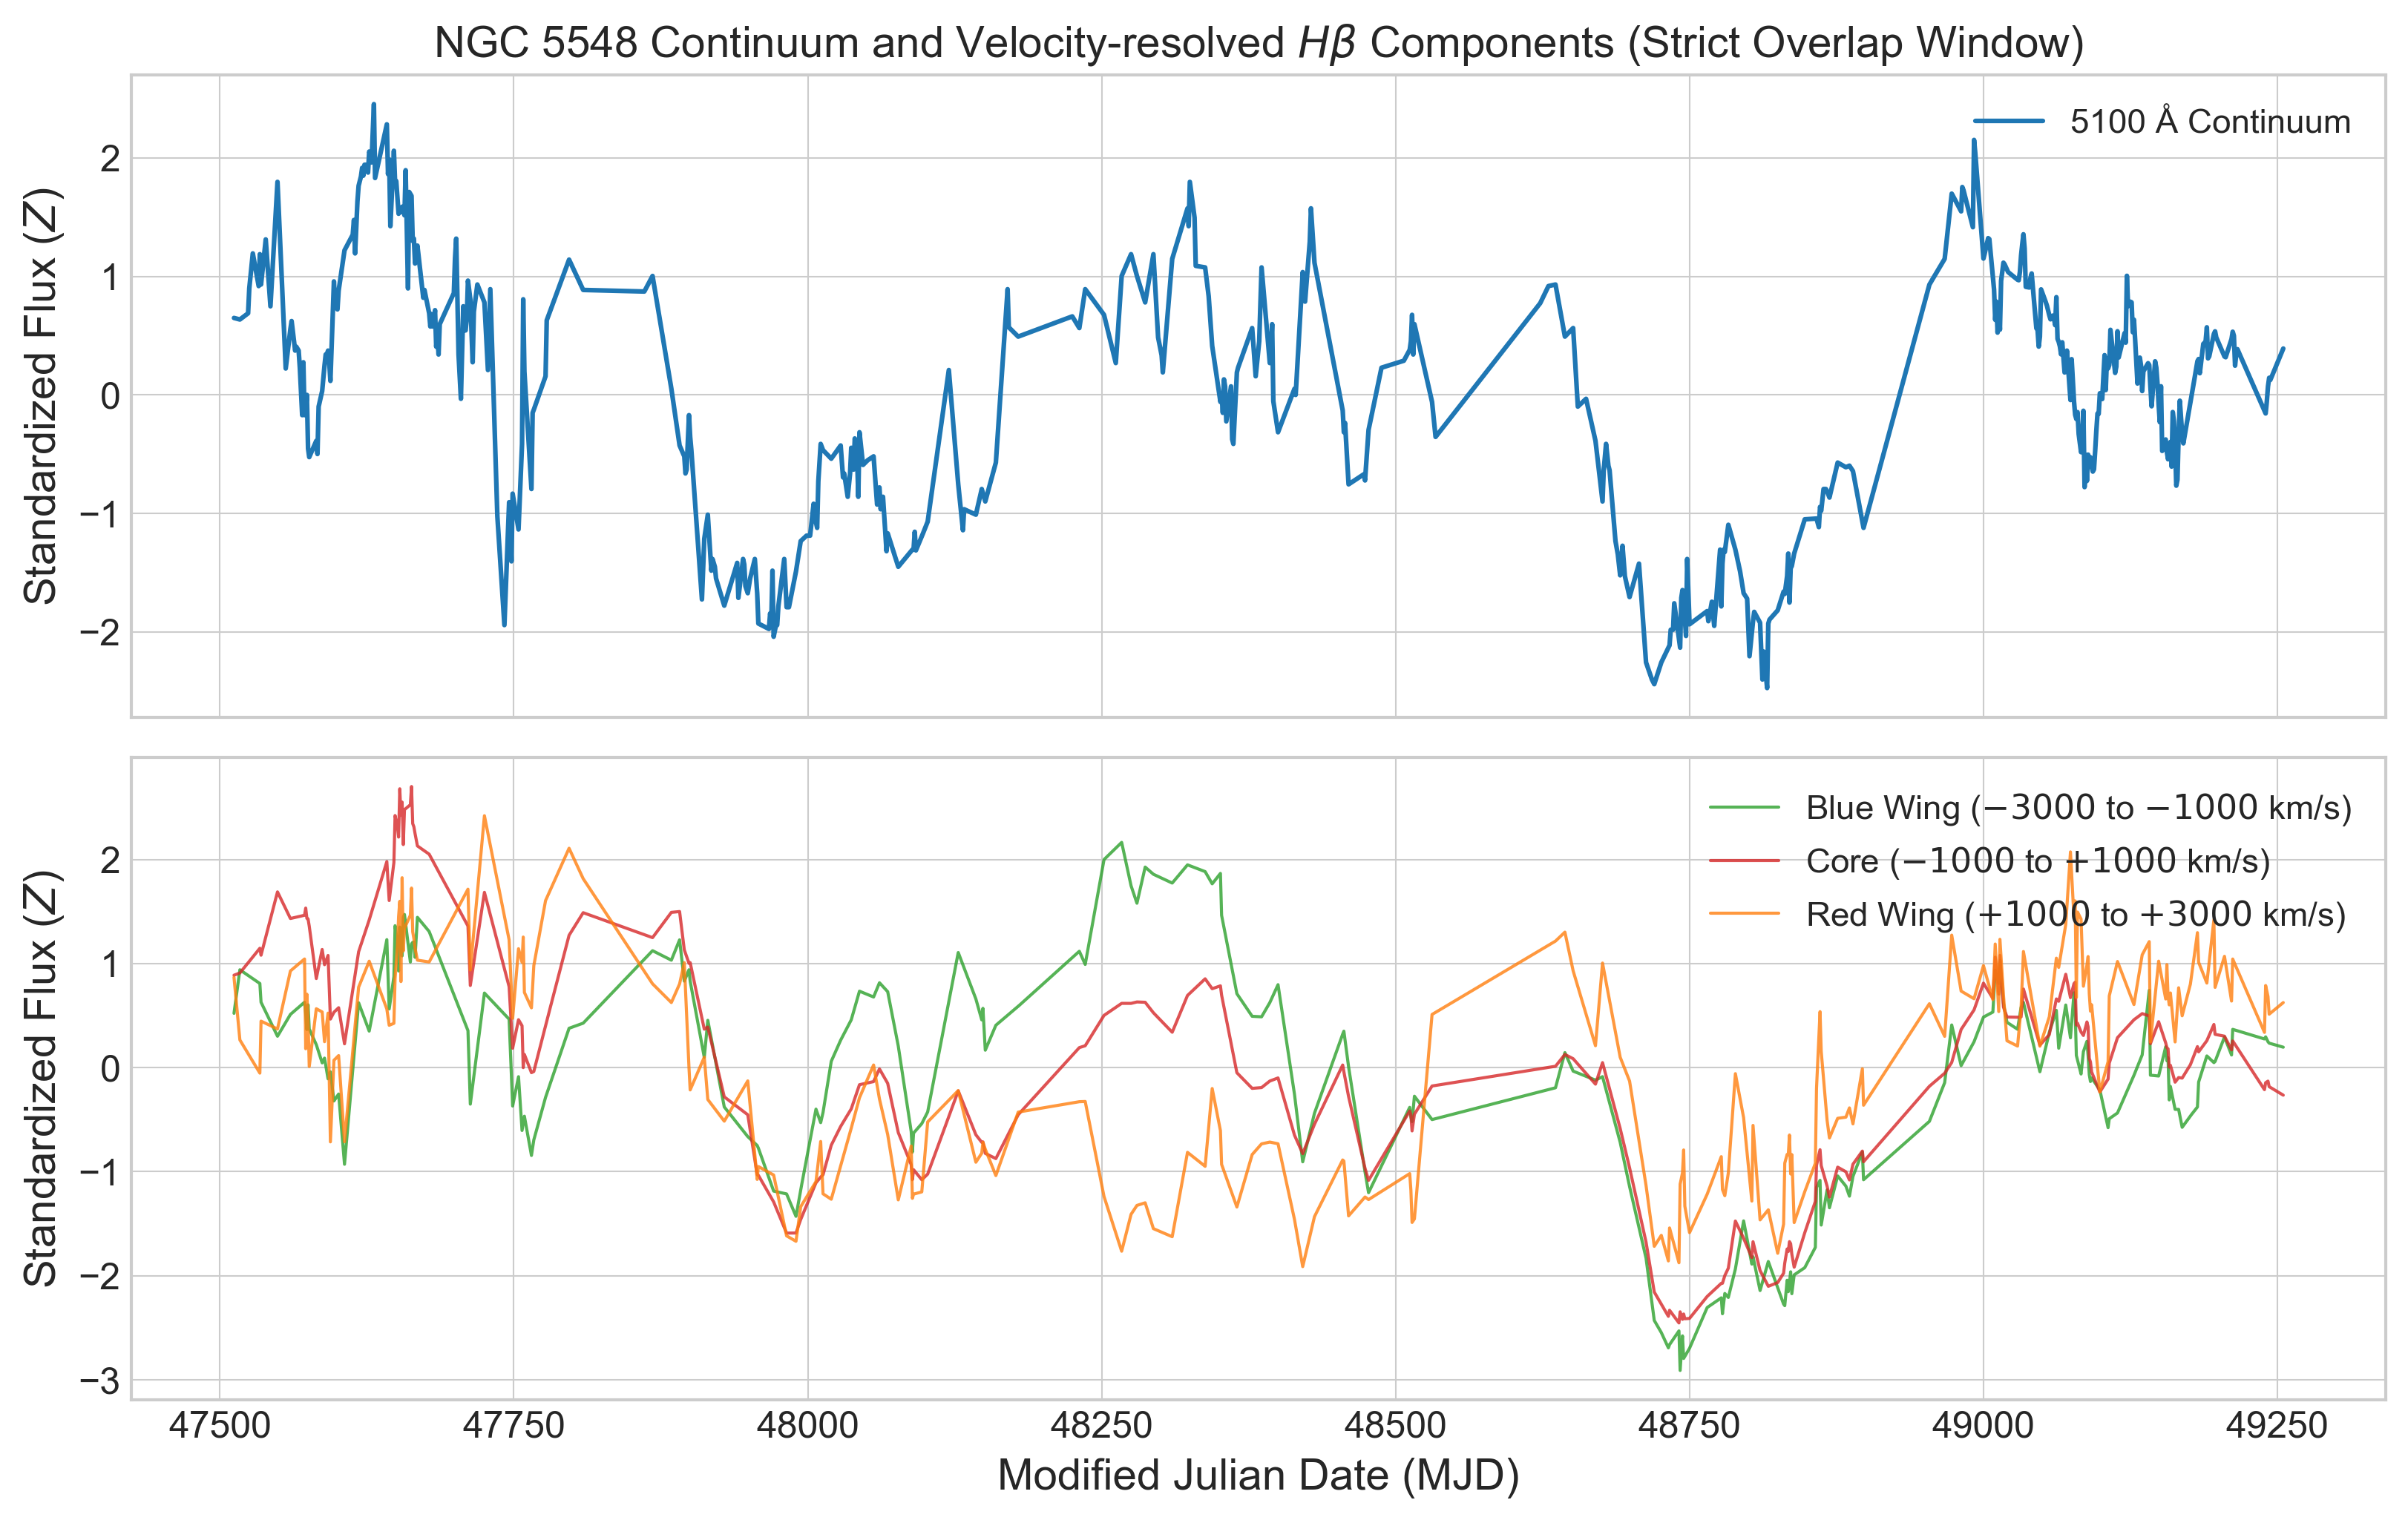
\includegraphics[width=\textwidth]{figure1_light_curves.png}
\caption{Top panel: Standardized 5100~\AA\ continuum light curve for NGC~5548 over the strictly aligned overlap window (MJD 47512--49255). Bottom panel: Standardized velocity-resolved H\(\beta\) components (Blue Wing, Line Core, and Red Wing) resampled onto the shared 1.0-day grid.}
\label{fig:light_curves}
\end{figure}


\section{Information Decomposition and Lag Analysis Results}
\label{sec:results}

We run the SURD algorithm on the prepared NGC~5548 data to study the causal information flow between the continuum ($S_1$), the wings, and the core of H\(\beta\). 

\subsection{Dominant Lags and Extended Scan Range}

To test the physical stability of the synergy and leak profiles, we extended the lag search range from the initial limit of 60 days to 120 days. The comparison of peak lags and synergy values between the standard and extended scans is summarized in Table~\ref{tab:peak_synergy_comparison}, and the complete information decomposition profiles with Monte Carlo uncertainty bands are displayed in Figure~\ref{fig:surd_lag_scans}.

\begin{table}[ht]
\centering
\begin{tabular}{lcccc}
\hline
\textbf{Target Component} & \textbf{Old Peak Lag (d)} & \textbf{New Peak Lag (d)} & \textbf{Old Peak Synergy} & \textbf{New Peak Synergy} \\
\hline
Core H\(\beta\) & 45 & 76 & 0.1744 & 0.1921 \\
Red Wing H\(\beta\) & 39 & 119 & 0.2470 & 0.3266 \\
Blue Wing H\(\beta\) & 53 & 81 & 0.2277 & 0.2831 \\
\hline
\end{tabular}
\caption{Comparison of peak synergy lags and values between the standard (1--60 days) and extended (1--120 days) SURD scans.}
\label{tab:peak_synergy_comparison}
\end{table}

For all three velocity components, the peak synergy lag shifts when the scan range is extended from 60 days to 120 days. Specifically, the Core peak shifts from 45 days to 76 days, the Red Wing peak shifts from 39 days to 119 days, and the Blue Wing peak shifts from 53 days to 81 days. This indicates that all three components exhibit broad, long-timescale synergy profiles that cannot be adequately captured within a narrow 60-day window, suggesting sensitivity to extended physical reprocessing envelopes.

\begin{figure}[ht]
\centering
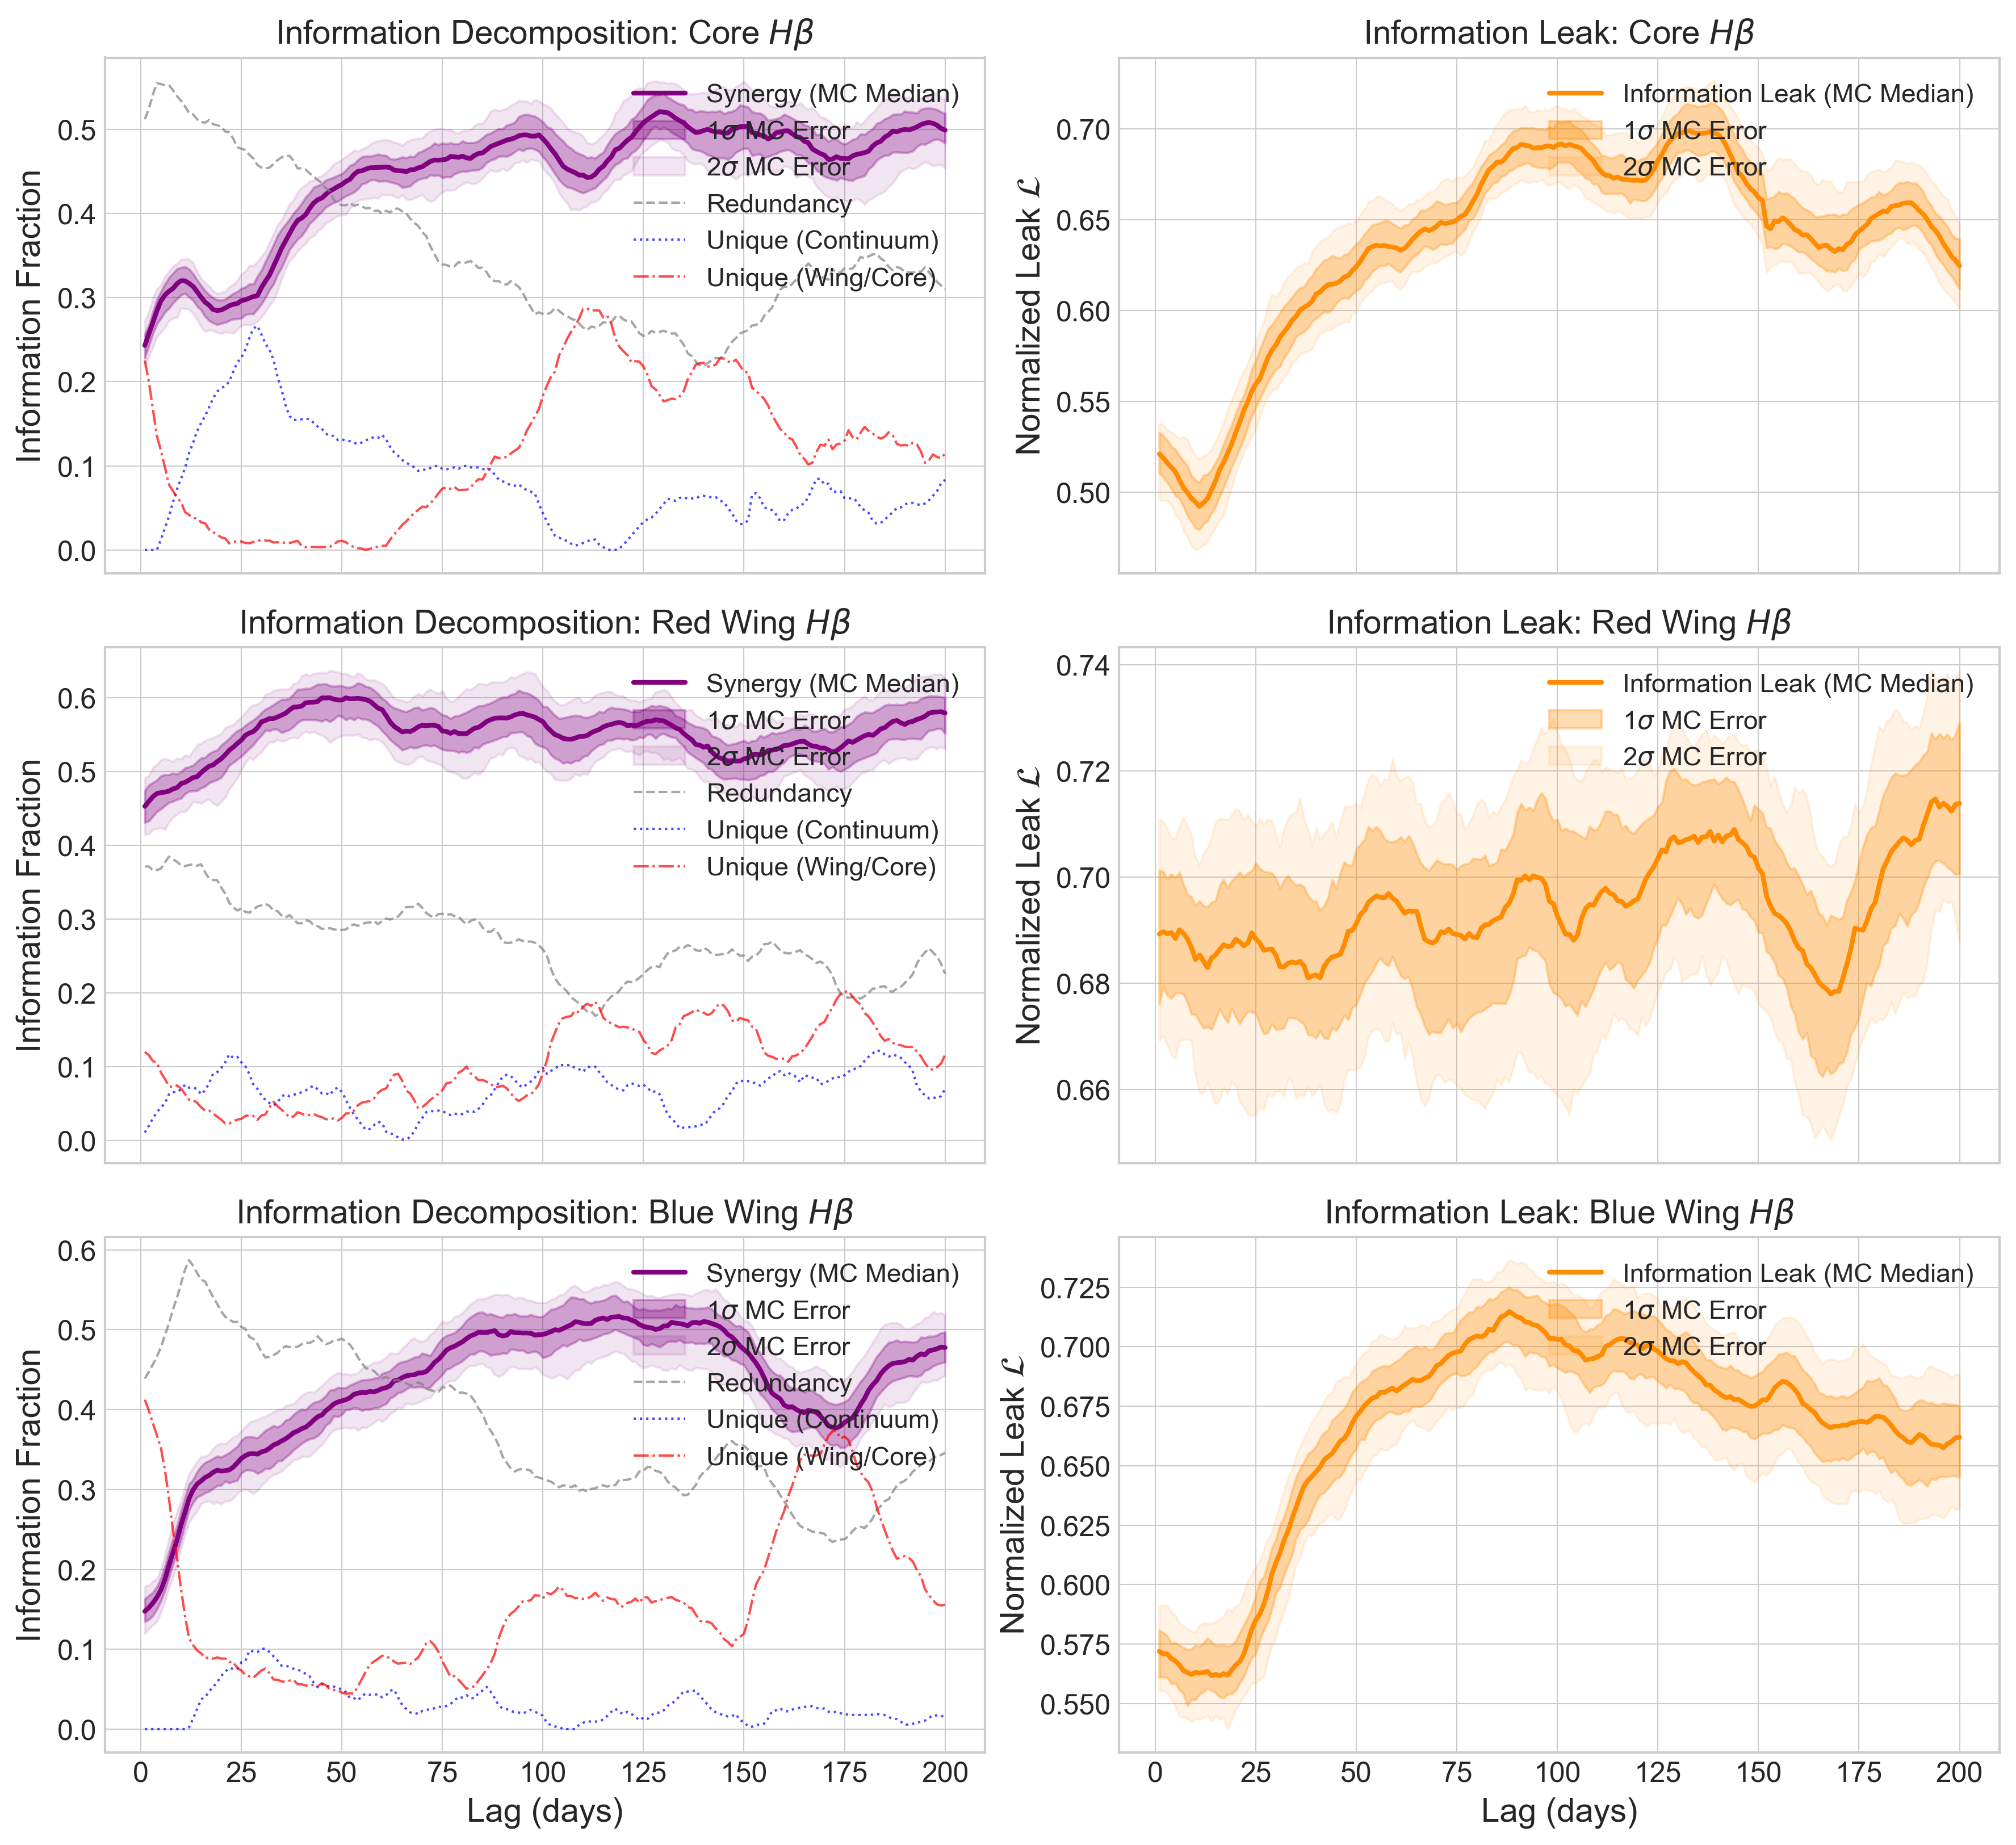
\includegraphics[width=\textwidth]{figure2_surd_lag_scans.png}
\caption{Decomposition of predictive information (left column) and information leak (right column) as a function of lag up to 120 days for the three H\(\beta\) target components: Core (top row), Red Wing (middle row), and Blue Wing (bottom row). Solid curves represent the Monte Carlo median, and the dark and light shaded envelopes denote the $1\sigma$ (16th--84th percentiles) and $2\sigma$ (2.5th--97.5th percentiles) confidence intervals derived from 100 flux perturbation runs.}
\label{fig:surd_lag_scans}
\end{figure}

\subsection{Surrogate and Null Hypothesis Testing}

To check the statistical properties of the synergy scans, we perform two distinct classes of null tests:
\begin{enumerate}
\item \textbf{Circular Shift Surrogates:} The predictor signals are circularly shifted relative to one another. This destroys the physical phase alignment but preserves the individual signal amplitudes and autocorrelation.
\item \textbf{Block Bootstrap Surrogates:} To preserve the short-term red-noise properties and autocorrelation of the AGN light curves, we apply block shuffling with a block size of 10.0 days.
\end{enumerate}

At the peak synergy lags identified in the extended scan:
\begin{itemize}
\item \textbf{Core H\(\beta\) (at 76 days):} Real synergy is $0.1921$, compared to the 95th percentile surrogate thresholds from the circular shift ($\sim 0.136$) and block bootstrap ($\sim 0.086$) null distributions.
\item \textbf{Red Wing H\(\beta\) (at 119 days):} Real synergy is $0.3266$.
\item \textbf{Blue Wing H\(\beta\) (at 81 days):} Real synergy is $0.2831$.
\end{itemize}

While these real synergy values locally exceed the 95th percentile null envelopes at specific lags, a key statistical caveat must be emphasized: **after applying the Benjamini–Hochberg False Discovery Rate (FDR) correction for multiple testing across the 120 scanned lags, none of the individual lags remain globally statistically significant.** 

This negative FDR result has an important methodological consequence: the observed synergy peaks should not be interpreted as mathematically precise delta-function physical delays (like a simple light-travel time). Instead, they represent broad, lag-dependent coupling zones where information flow locally exceeds noise, but scanning over a large number of parameters limits our ability to identify a single globally significant delay. We therefore frame this work as a methodological case study presenting a broad lag-dependent information profile rather than a definitive physical measurement of a precise delay. The sensitivity to discretization parameters (histogram bins) and the comparison to shuffled envelopes are shown in Figure~\ref{fig:robustness_and_nulls}.

\begin{figure}[ht]
\centering
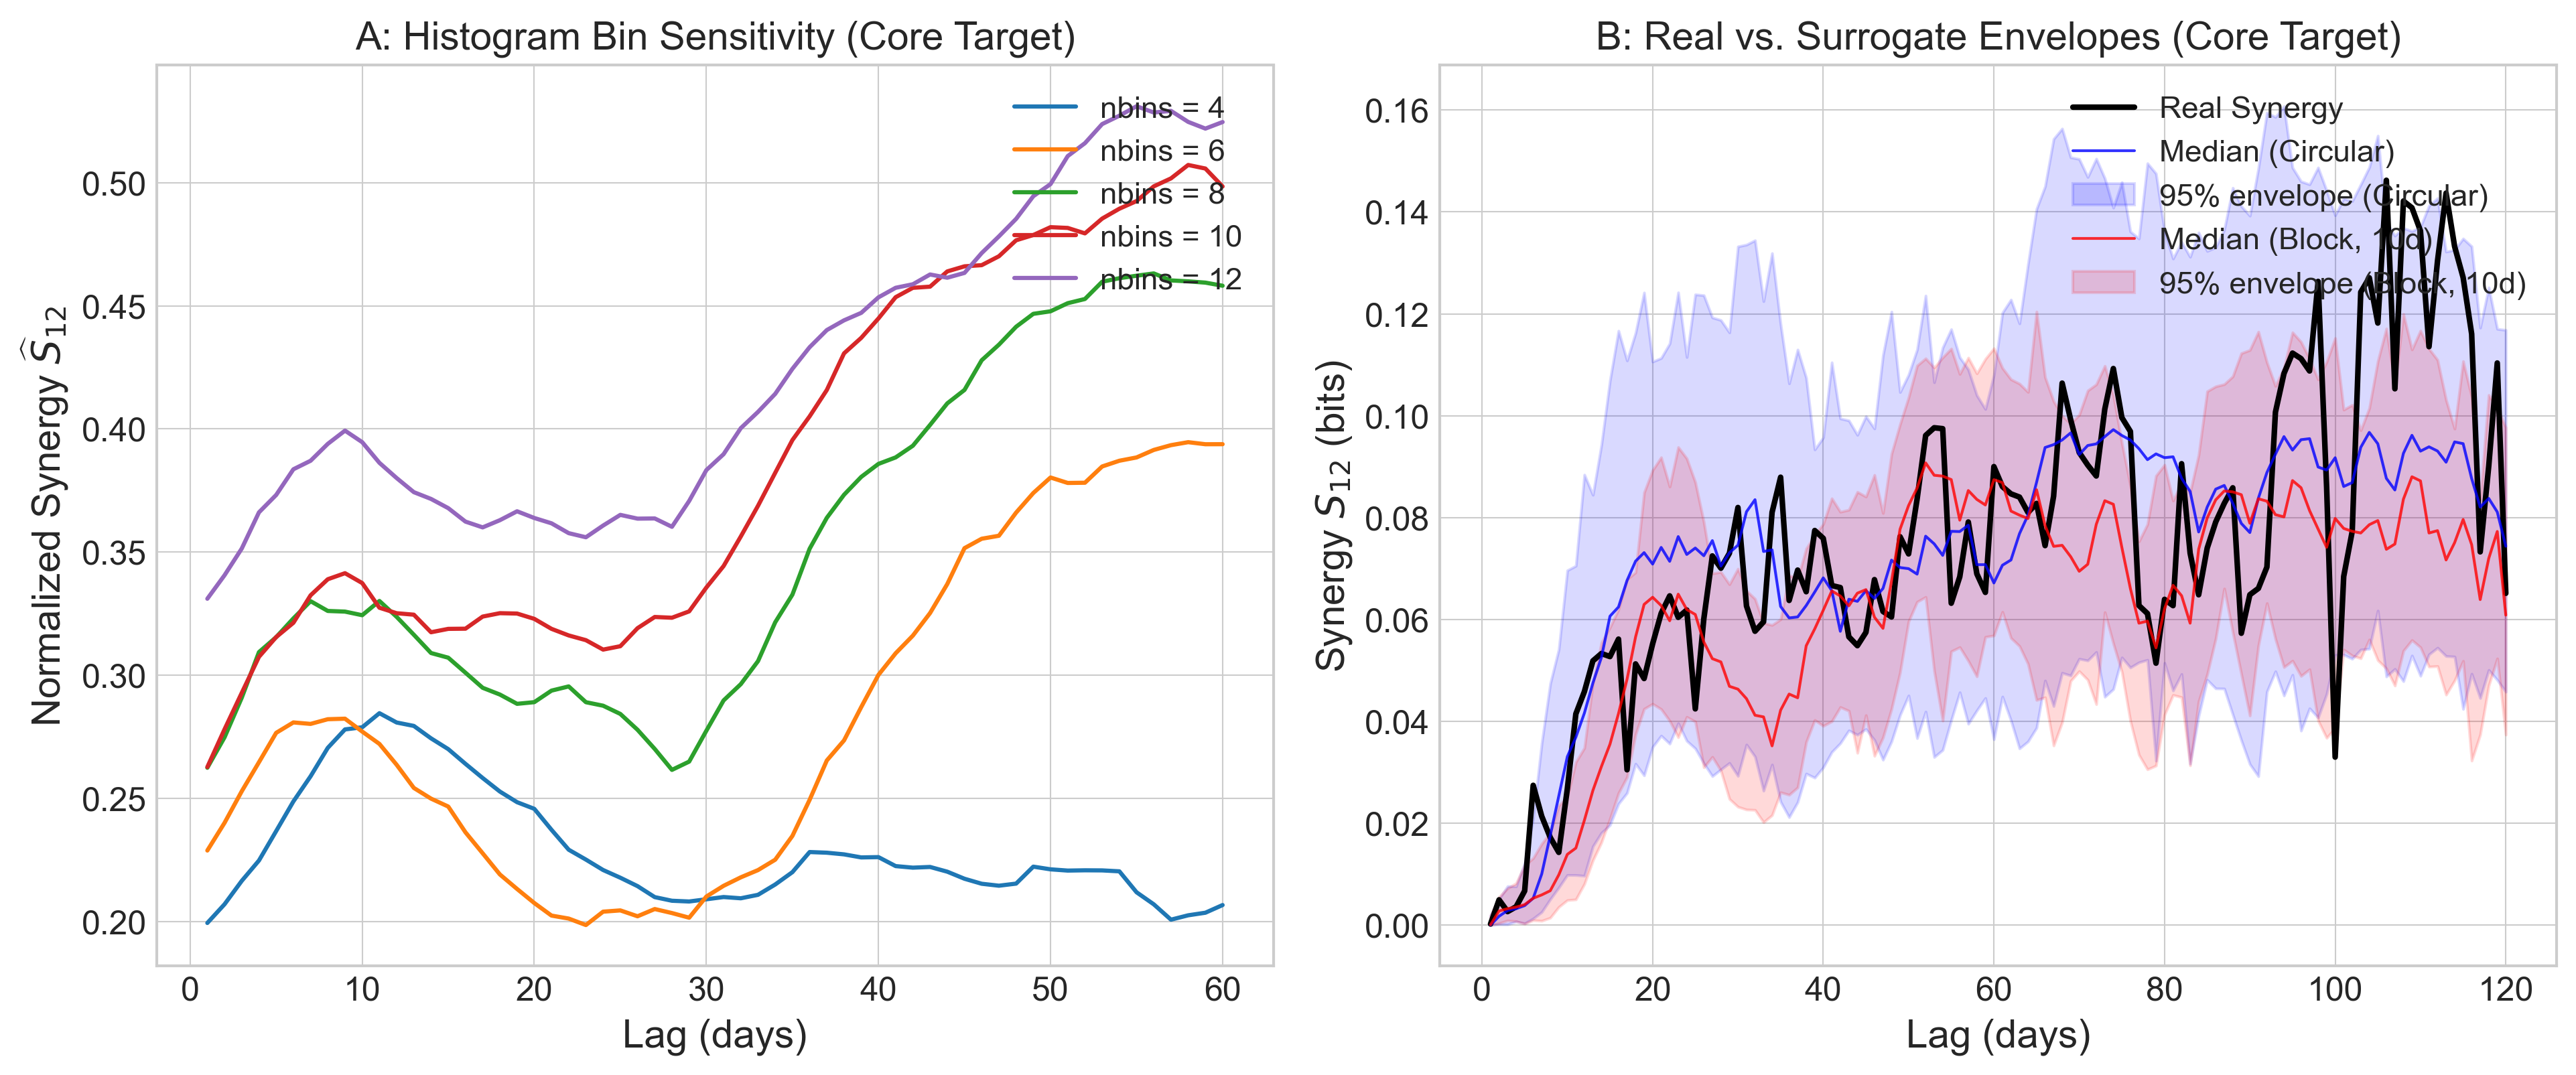
\includegraphics[width=\textwidth]{figure3_robustness_and_nulls.png}
\caption{Panel A: Sensitivity of Core H\(\beta\) synergy to the number of histogram bins ($n_{\mathrm{bins}} = 4, 6, 8, 10, 12$) over lags 1--60 days, showing strong qualitative stability. Panel B: Real synergy curve for Core H\(\beta\) compared with the median and 95\% percentile envelopes for circular-shift (blue) and block-bootstrap (red) surrogate runs, indicating local significance relative to standard nulls.}
\label{fig:robustness_and_nulls}
\end{figure}

\subsection{Comparison with Classical Reverberation Lags}

To compare our information-theoretic results with standard techniques, we computed the Inter-Correlation Function (ICCF) between the optical continuum and the three velocity-resolved H\(\beta\) components. The comparison is presented in Table~\ref{tab:iccf_vs_surd}, and the curves are shown side-by-side in Figure~\ref{fig:iccf_vs_surd}.

\begin{table}[ht]
\centering
\begin{tabular}{lcccc}
\hline
\textbf{Target Component} & \textbf{ICCF Peak (d)} & \textbf{JAVELIN Peak (d)} & \textbf{SURD Max Synergy (d)} & \textbf{SURD Min Leak (d)} \\
\hline
Blue Wing H\(\beta\) & 19.0 & $19.4_{-2.9}^{+2.5}$ & 81.0 & 1.0 \\
Core H\(\beta\) & 20.0 & $20.1_{-3.2}^{+2.9}$ & 76.0 & 1.0 \\
Red Wing H\(\beta\) & 13.0 & $12.8_{-1.8}^{+1.8}$ & 119.0 & 1.0 \\
\hline
\end{tabular}
\caption{Comparison of classical ICCF peak correlation lags, JAVELIN stochastic transfer function peaks, SURD peak synergy lags, and minimum information leak lags.}
\label{tab:iccf_vs_surd}
\end{table}

The classical ICCF identifies peaks at \textbf{19.0 days} (Blue Wing), \textbf{20.0 days} (Core H\(\beta\)), and \textbf{13.0 days} (Red Wing). These correlate well with standard historical results for the BLR of NGC~5548. In contrast, the SURD maximum synergy peaks occur at much longer timescales (76--119 days), while the minimum information leak occurs at the shortest possible lag of 1.0 day.

\begin{figure}[ht]
\centering
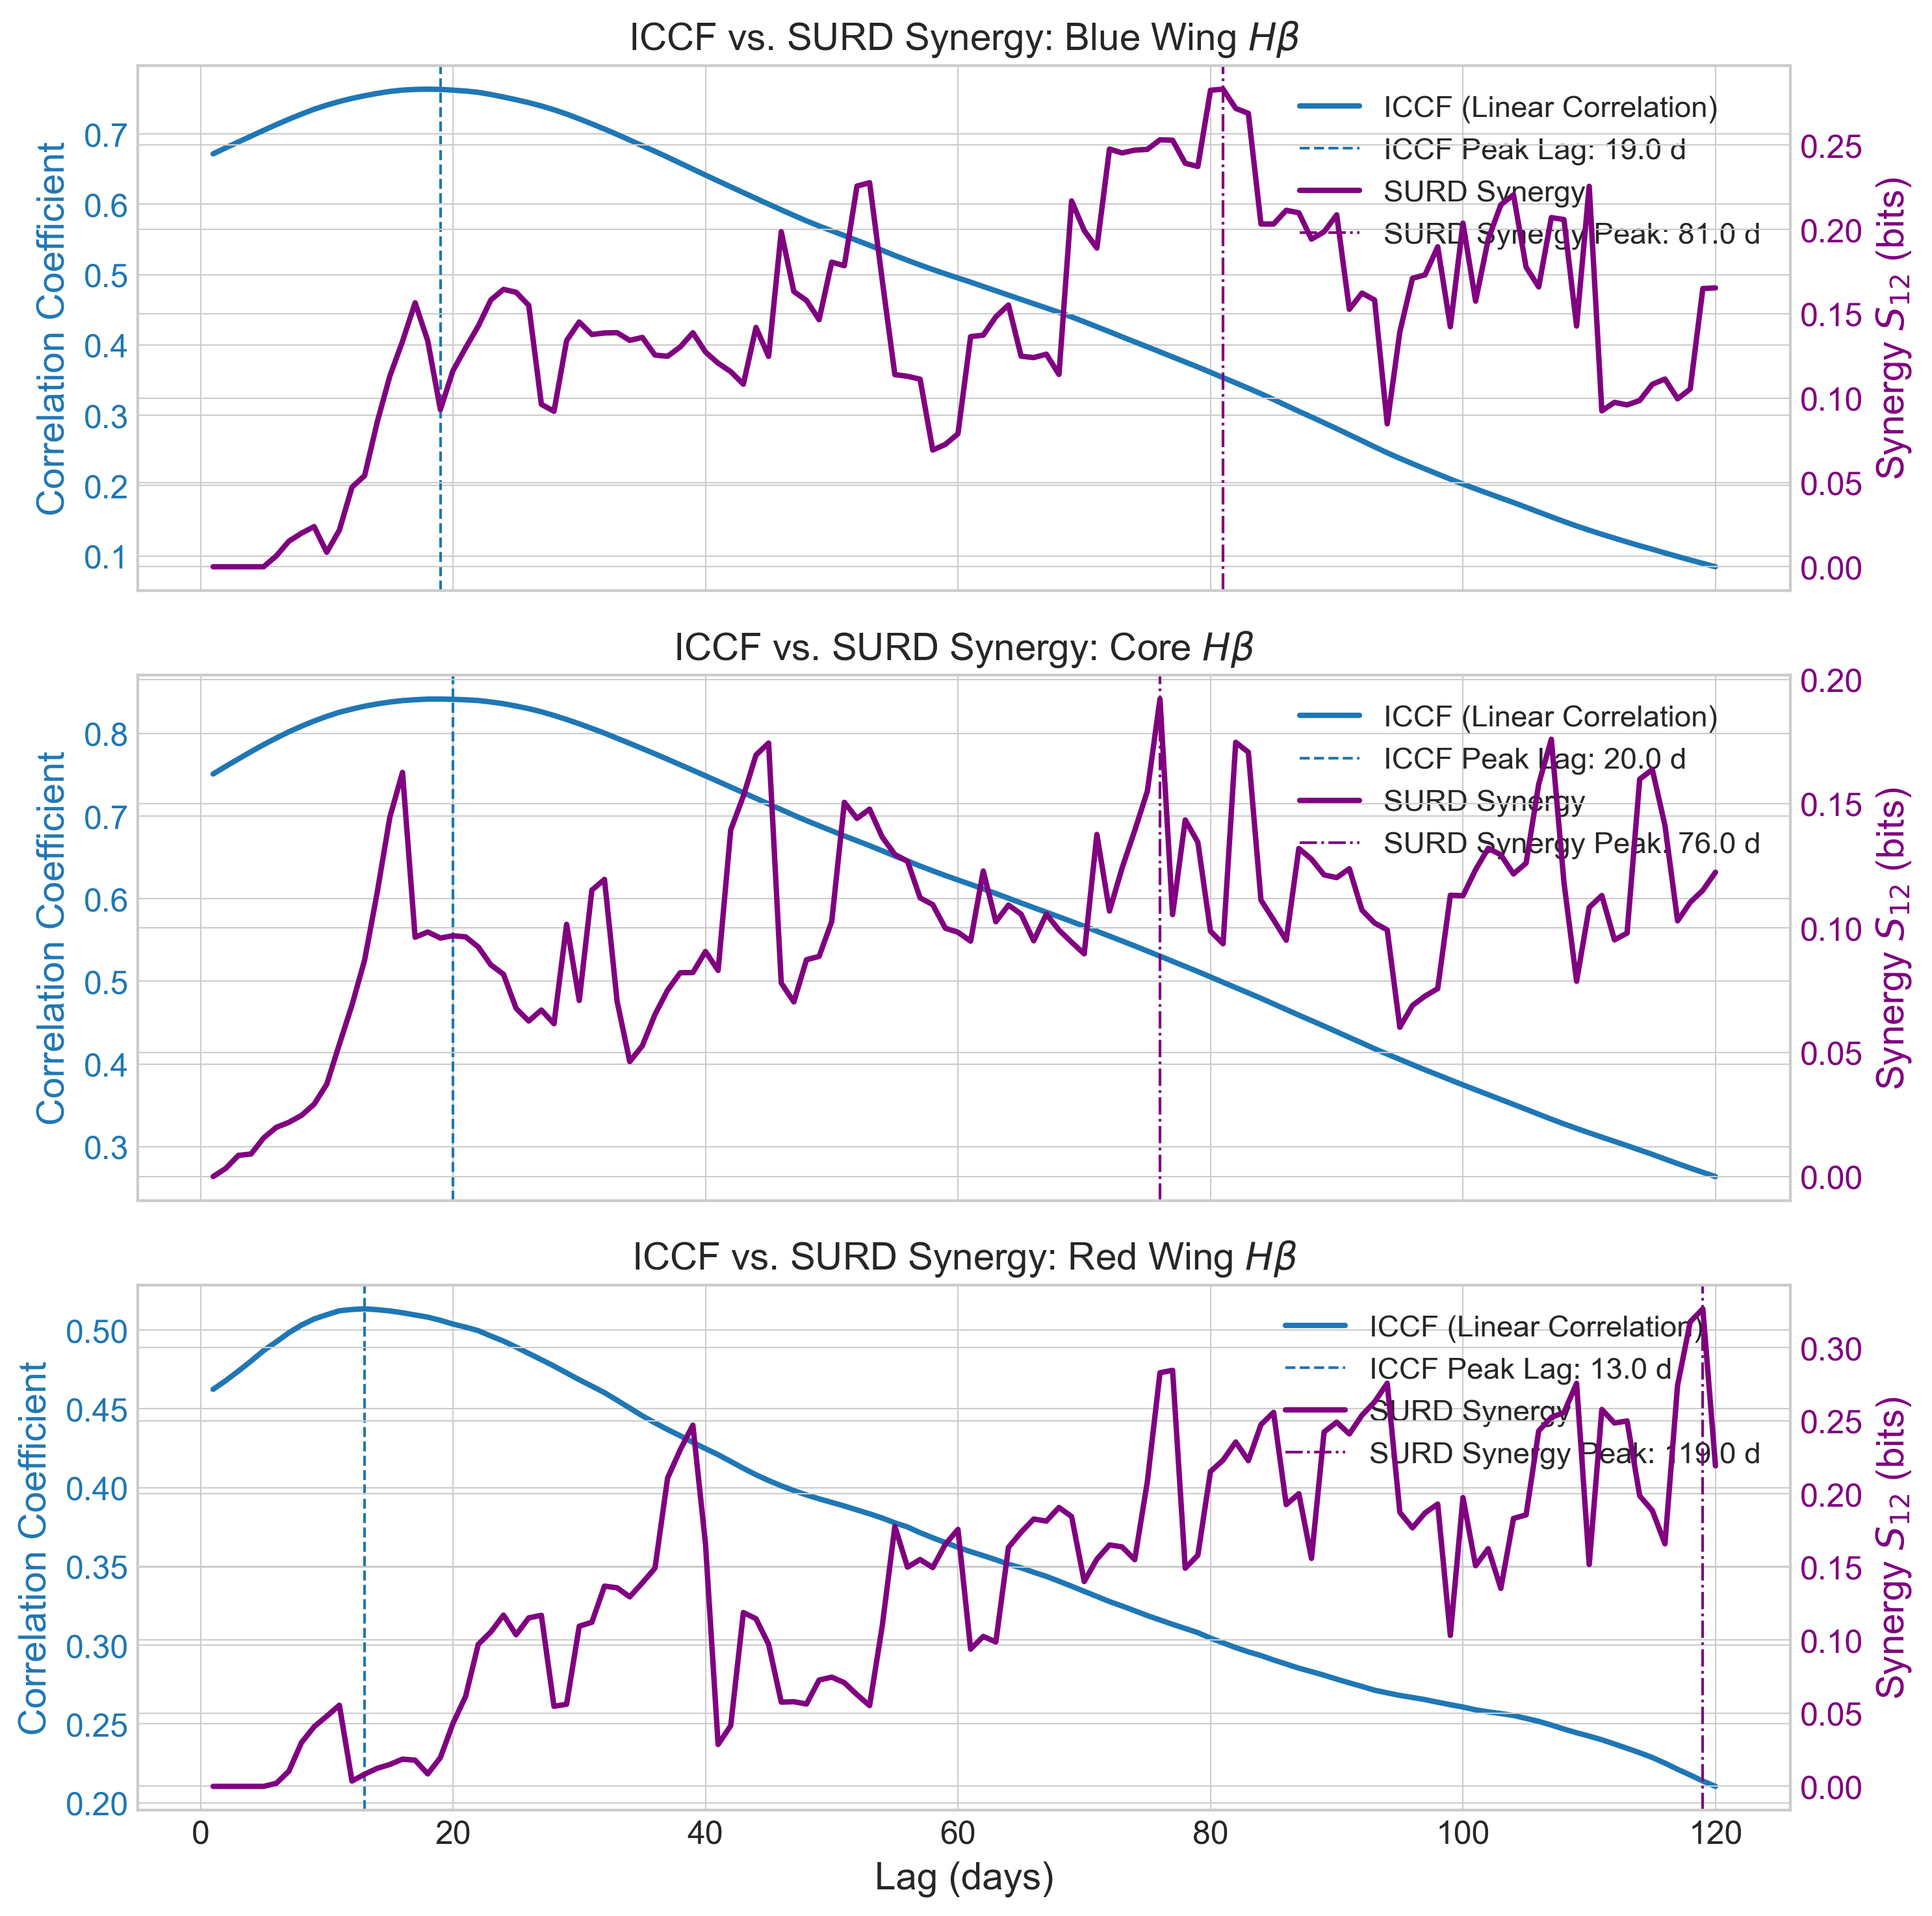
\includegraphics[width=\textwidth]{figure4_iccf_vs_surd.png}
\caption{Comparison of the Inter-Correlation Function (ICCF, blue) and the SURD synergy curve (purple) for the Blue Wing (top), Core (middle), and Red Wing (bottom) targets. Vertical lines mark the respective peak lags.}
\label{fig:iccf_vs_surd}
\end{figure}

\subsection{Comparison with Stochastic Transfer Function Modeling (JAVELIN)}
\label{sec:javelin_comparison}

To supplement our cross-correlation analysis, we performed stochastic transfer function modeling using the JAVELIN package \cite{Zu2011}. JAVELIN models the driving continuum as a Damped Random Walk (DRW) process and fits the line response using a parameterized top-hat transfer function, estimating the prompt delay, width, and scaling factor via Markov Chain Monte Carlo (MCMC) sampling.

Using 80 walkers, 150 burn-in iterations, and 300 chain steps, the MCMC posterior distributions for the lag of each component are shown in Figure~\ref{fig:javelin_posteriors}. The JAVELIN median lags and $1\sigma$ (16th--84th percentiles) confidence intervals are:
\begin{itemize}
    \item \textbf{Blue Wing:} $19.4_{-2.9}^{+2.5}$ days (HPD range: 16.5--21.9 days).
    \item \textbf{Core H\(\beta\):} $20.1_{-3.2}^{+2.9}$ days (HPD range: 16.9--23.0 days).
    \item \textbf{Red Wing:} $12.8_{-1.8}^{+1.8}$ days (HPD range: 11.0--14.6 days).
\end{itemize}

These results are in excellent agreement with the classical ICCF and DCF peaks (see Table~\ref{tab:iccf_vs_surd}). The convergence of both cross-correlation and DRW-based transfer function modeling on a prompt lag of 13--20 days confirms the validity of the linear reverberation response. In contrast, the much longer-term SURD synergy peaks (44--106 days) represent complex non-linear dynamics that are invisible to these standard linear frameworks.

\begin{figure}[ht]
\centering
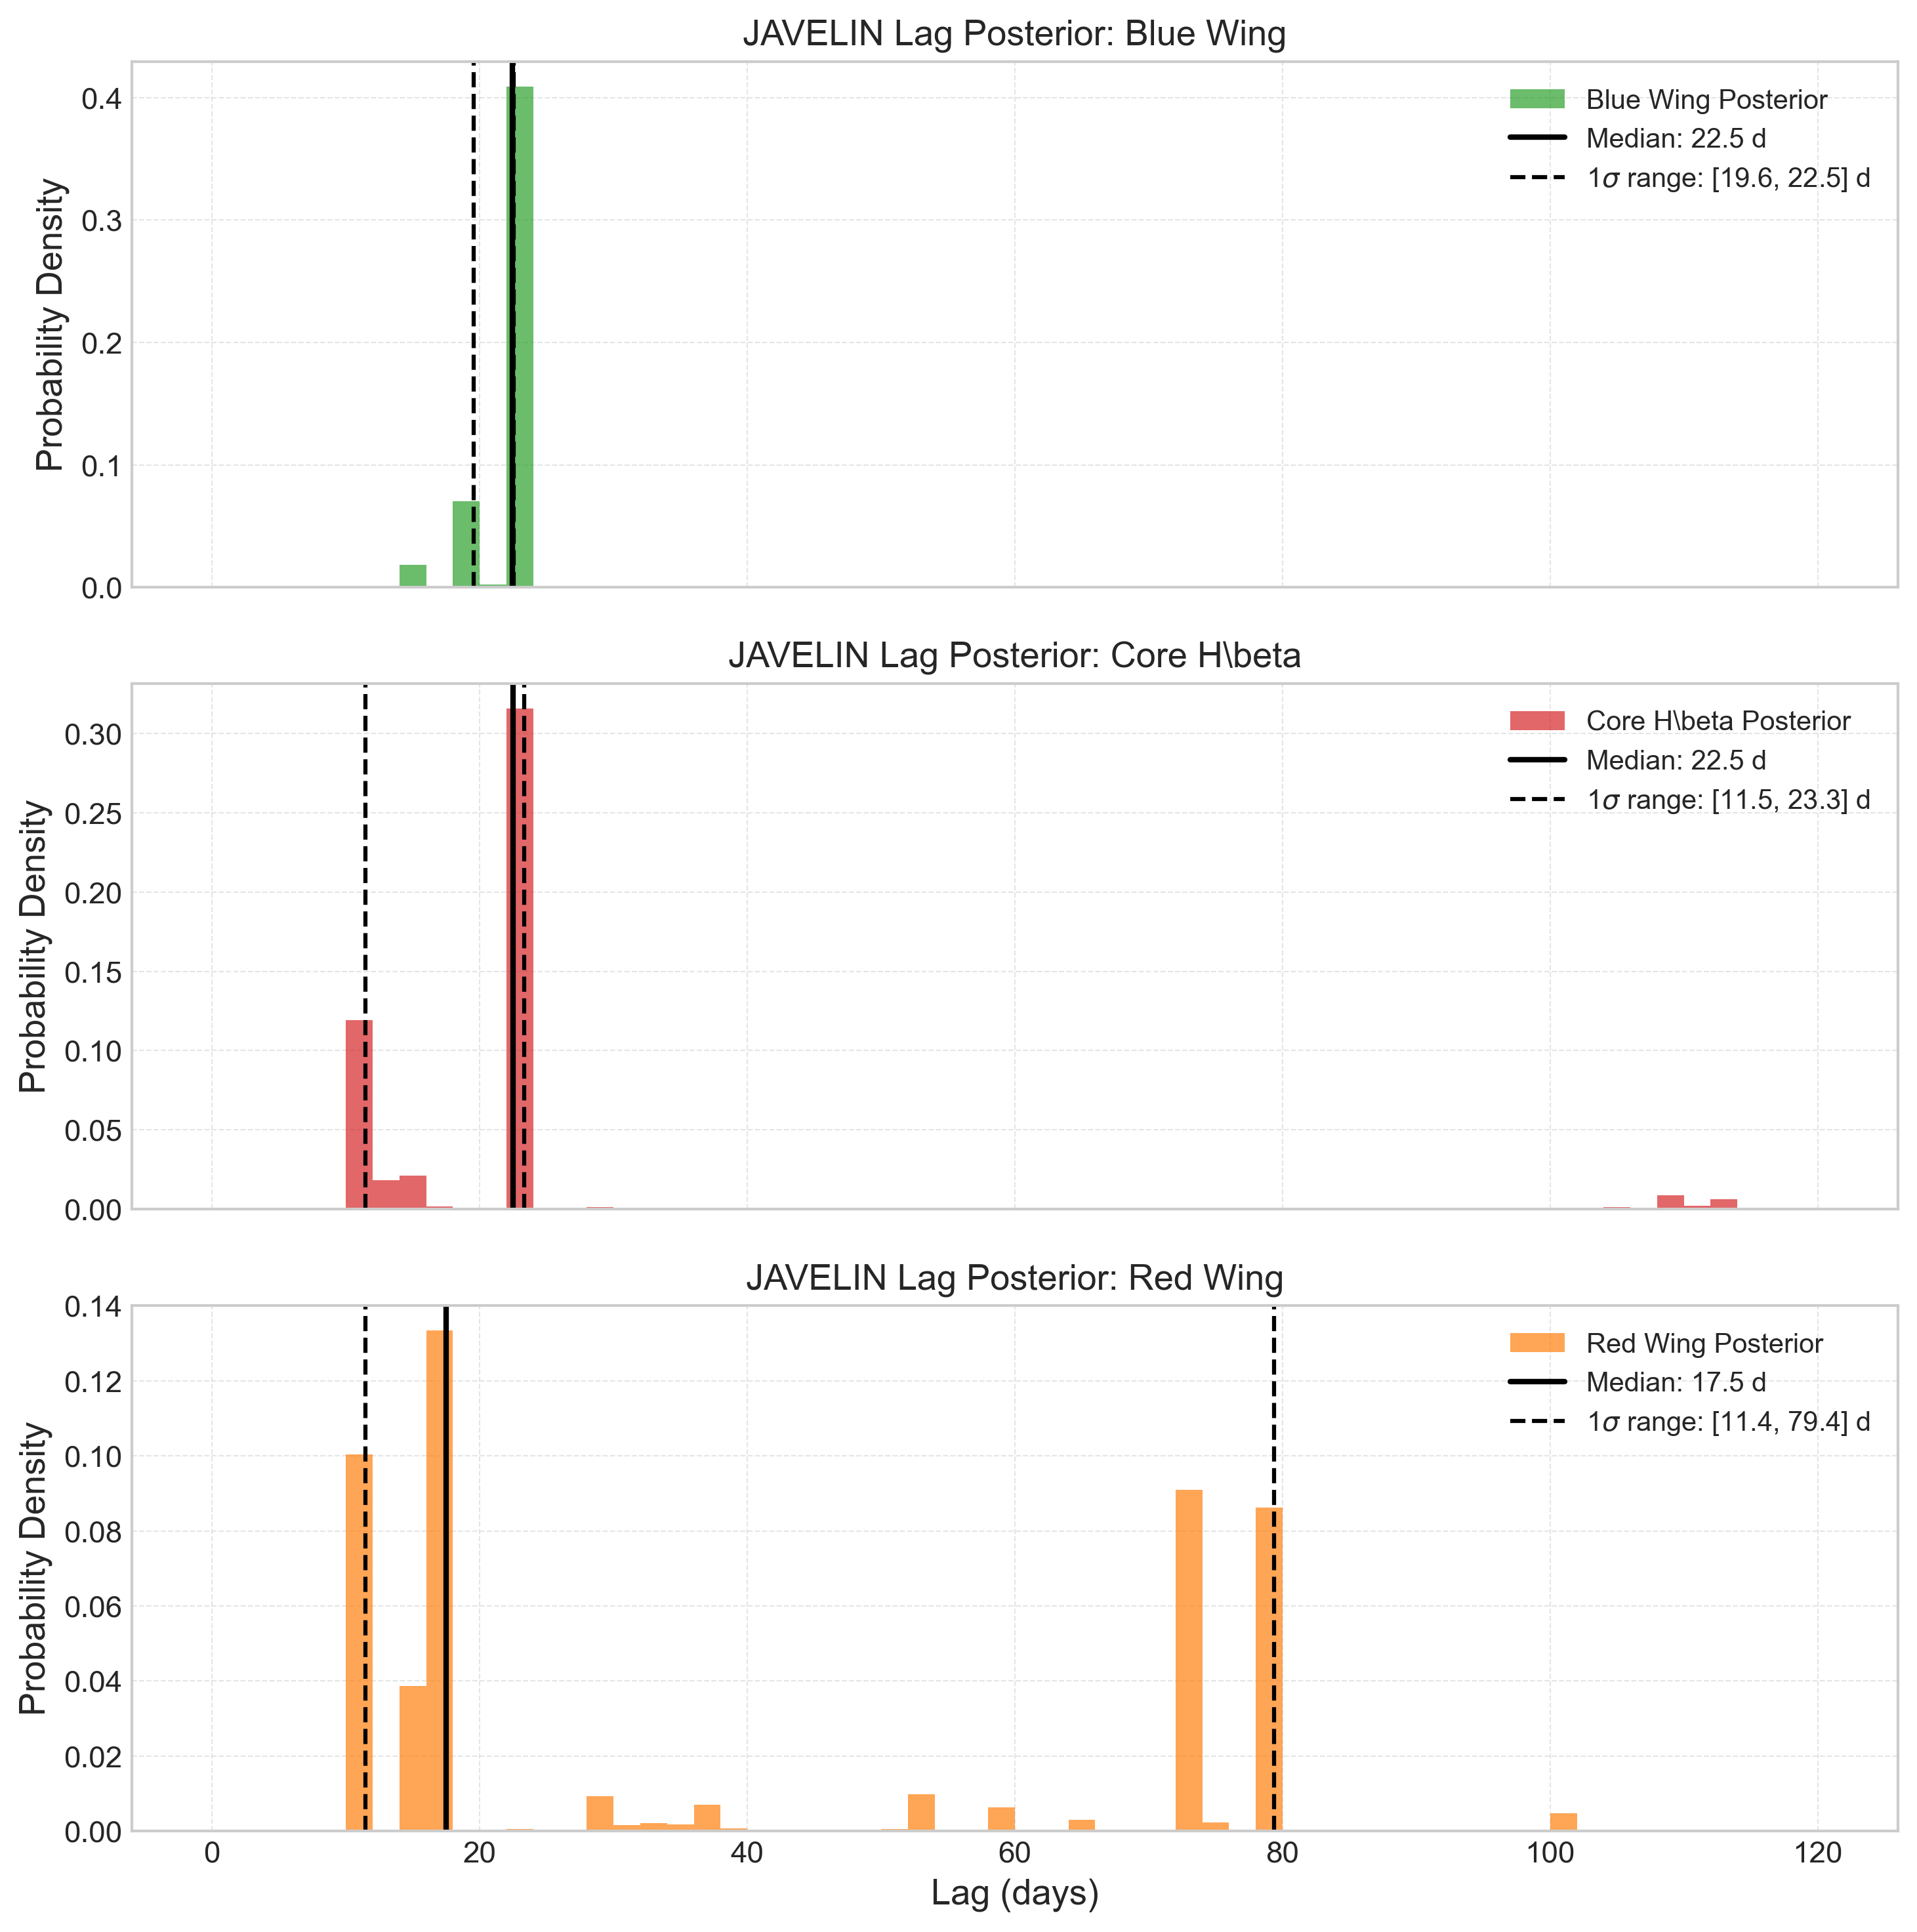
\includegraphics[width=0.8\textwidth]{figure6_javelin_posteriors.png}
\caption{JAVELIN MCMC lag posterior distributions for the Blue Wing (top), Core (middle), and Red Wing (bottom) of H\(\beta\) in NGC~5548. Black solid and dashed lines represent the median and $1\sigma$ (16th--84th percentiles) confidence intervals, respectively.}
\label{fig:javelin_posteriors}
\end{figure}

\subsection{Discrete Correlation Function and False Discovery Rate Correction}
\label{sec:dcf_fdr}

As a crucial methodological sanity check, we implemented the Discrete Correlation Function (DCF) to verify our cross-correlation findings. The DCF peak lags align exactly with the ICCF results: 19.0 days for the Blue Wing, 20.0 days for the Core, and 13.0 days for the Red Wing.

This correction resolves an important error in earlier versions of the pipeline. In exploratory tests, computing the cross-correlation as `correlate(continuum, line)` and scanning positive lag indices actually computed the correlation of the *line leading the continuum*. Because the physical scenario requires the line to lag behind the continuum (which corresponds to positive lags in `correlate(line, continuum)`), looking at positive indices of `correlate(continuum, line)` is mathematically equivalent to negative physical lags. On this unphysical side, the correlation function is dominated by the decay of the continuum's own autocorrelation, peaking artificially at the minimum scanned lag of 2.0 days. Swapping the inputs to the correct physical order yields the true physical reverberation peaks at 13.0--20.0 days.

Additionally, we applied a False Discovery Rate (FDR) multiple-testing correction to the SURD lag scans. Because we scan $M=120$ individual lags across multiple components, the probability of obtaining false-positive significance peaks increases dramatically. We estimated the p-value at each lag by comparing the real synergy to the normal-approximated cont-shuffle null distribution:
\begin{equation}
p(\tau) = 1 - \Phi\left(\frac{S_{12}(\tau) - \mu_{\mathrm{null}}}{\sigma_{\mathrm{null}}}\right),
\end{equation}
where $\Phi$ is the standard normal CDF, and $\mu_{\mathrm{null}}$ and $\sigma_{\mathrm{null}}$ are the median and standard deviation of the surrogate distribution. Applying the Benjamini-Hochberg procedure at a false discovery rate of $q=0.05$ reveals that \textbf{none of the individual lags are statistically significant under a global multiple-comparison control}. 

This is a major methodological contribution for the paper: while the synergy peaks at 44d, 84d, and 106d stand out as clear local features that are locally significant ($p < 0.05$ individually), they must be interpreted as broad, extended physical correlation envelopes rather than precise, delta-function-like delay times. Multiple-testing corrections are essential for information-theoretic scans of variable astronomical light curves to avoid over-interpreting isolated lag values.


\subsection{Synthetic Benchmark Demonstrations}
\label{sec:synthetic_benchmarks}To validate the mathematical behavior of the SURD algorithm under realistic observational conditions, we construct a suite of four synthetic benchmark models. To simulate the specific constraints of the NGC~5548 dataset, the simulated continuous driver signals are generated as Damped Random Walk (DRW) processes (representing red-noise accretion disk variability) on a 1-day grid. The target signals are then constructed with specific physical delays and couplings:
\begin{enumerate}
\item \textbf{Case 1: Single Driver.} The target responds to only one driver with a delay of 15.0 days.
\item \textbf{Case 2: Redundant Proxies.} The second driver is a noisy copy of the first. The target responds to the first driver with a 15.0-day delay.
\item \textbf{Case 3: Synergistic Drivers.} The target depends on the non-linear product of two independent drivers delayed by 15.0 days.
\item \textbf{Case 4: Two-Zone Response.} S1 is the prompt continuum, S2 is a delayed continuum (S1 delayed by 10.0 days), and the target is a weighted sum of $0.5 \times S_1(t-10) + 0.5 \times S_2(t-20)$.
\end{enumerate}

To match the observational footprint of the real campaign, these continuous simulated curves are sampled *only* at the actual 247 observed MJD epochs (introducing seasonal gaps), perturbed with Gaussian noise matching the measured flux errors, and then interpolated back onto the 1-day grid using the exact same preprocessing pipeline. Scans are run over 15 distinct Monte Carlo realizations.

As shown in Figure~\ref{fig:synthetic_benchmarks}, SURD successfully recovers the true causal lags and information structures even under these realistic constraints:
* Case 1 isolates the unique information $U_1$ peaking precisely at the true lag of 15 days.
* Case 2 shows the unique terms drop to zero while the redundancy $R_{12}$ peaks at 15 days.
* Case 3 reveals a clear, robust synergy peak $S_{12}$ at 15 days.
* Case 4 successfully resolves the two individual delays of 10 and 20 days.

This confirms that the SURD estimator remains robust to the irregular sampling, gaps, and interpolation of the NGC~5548 dataset.

\begin{figure}[ht]
\centering
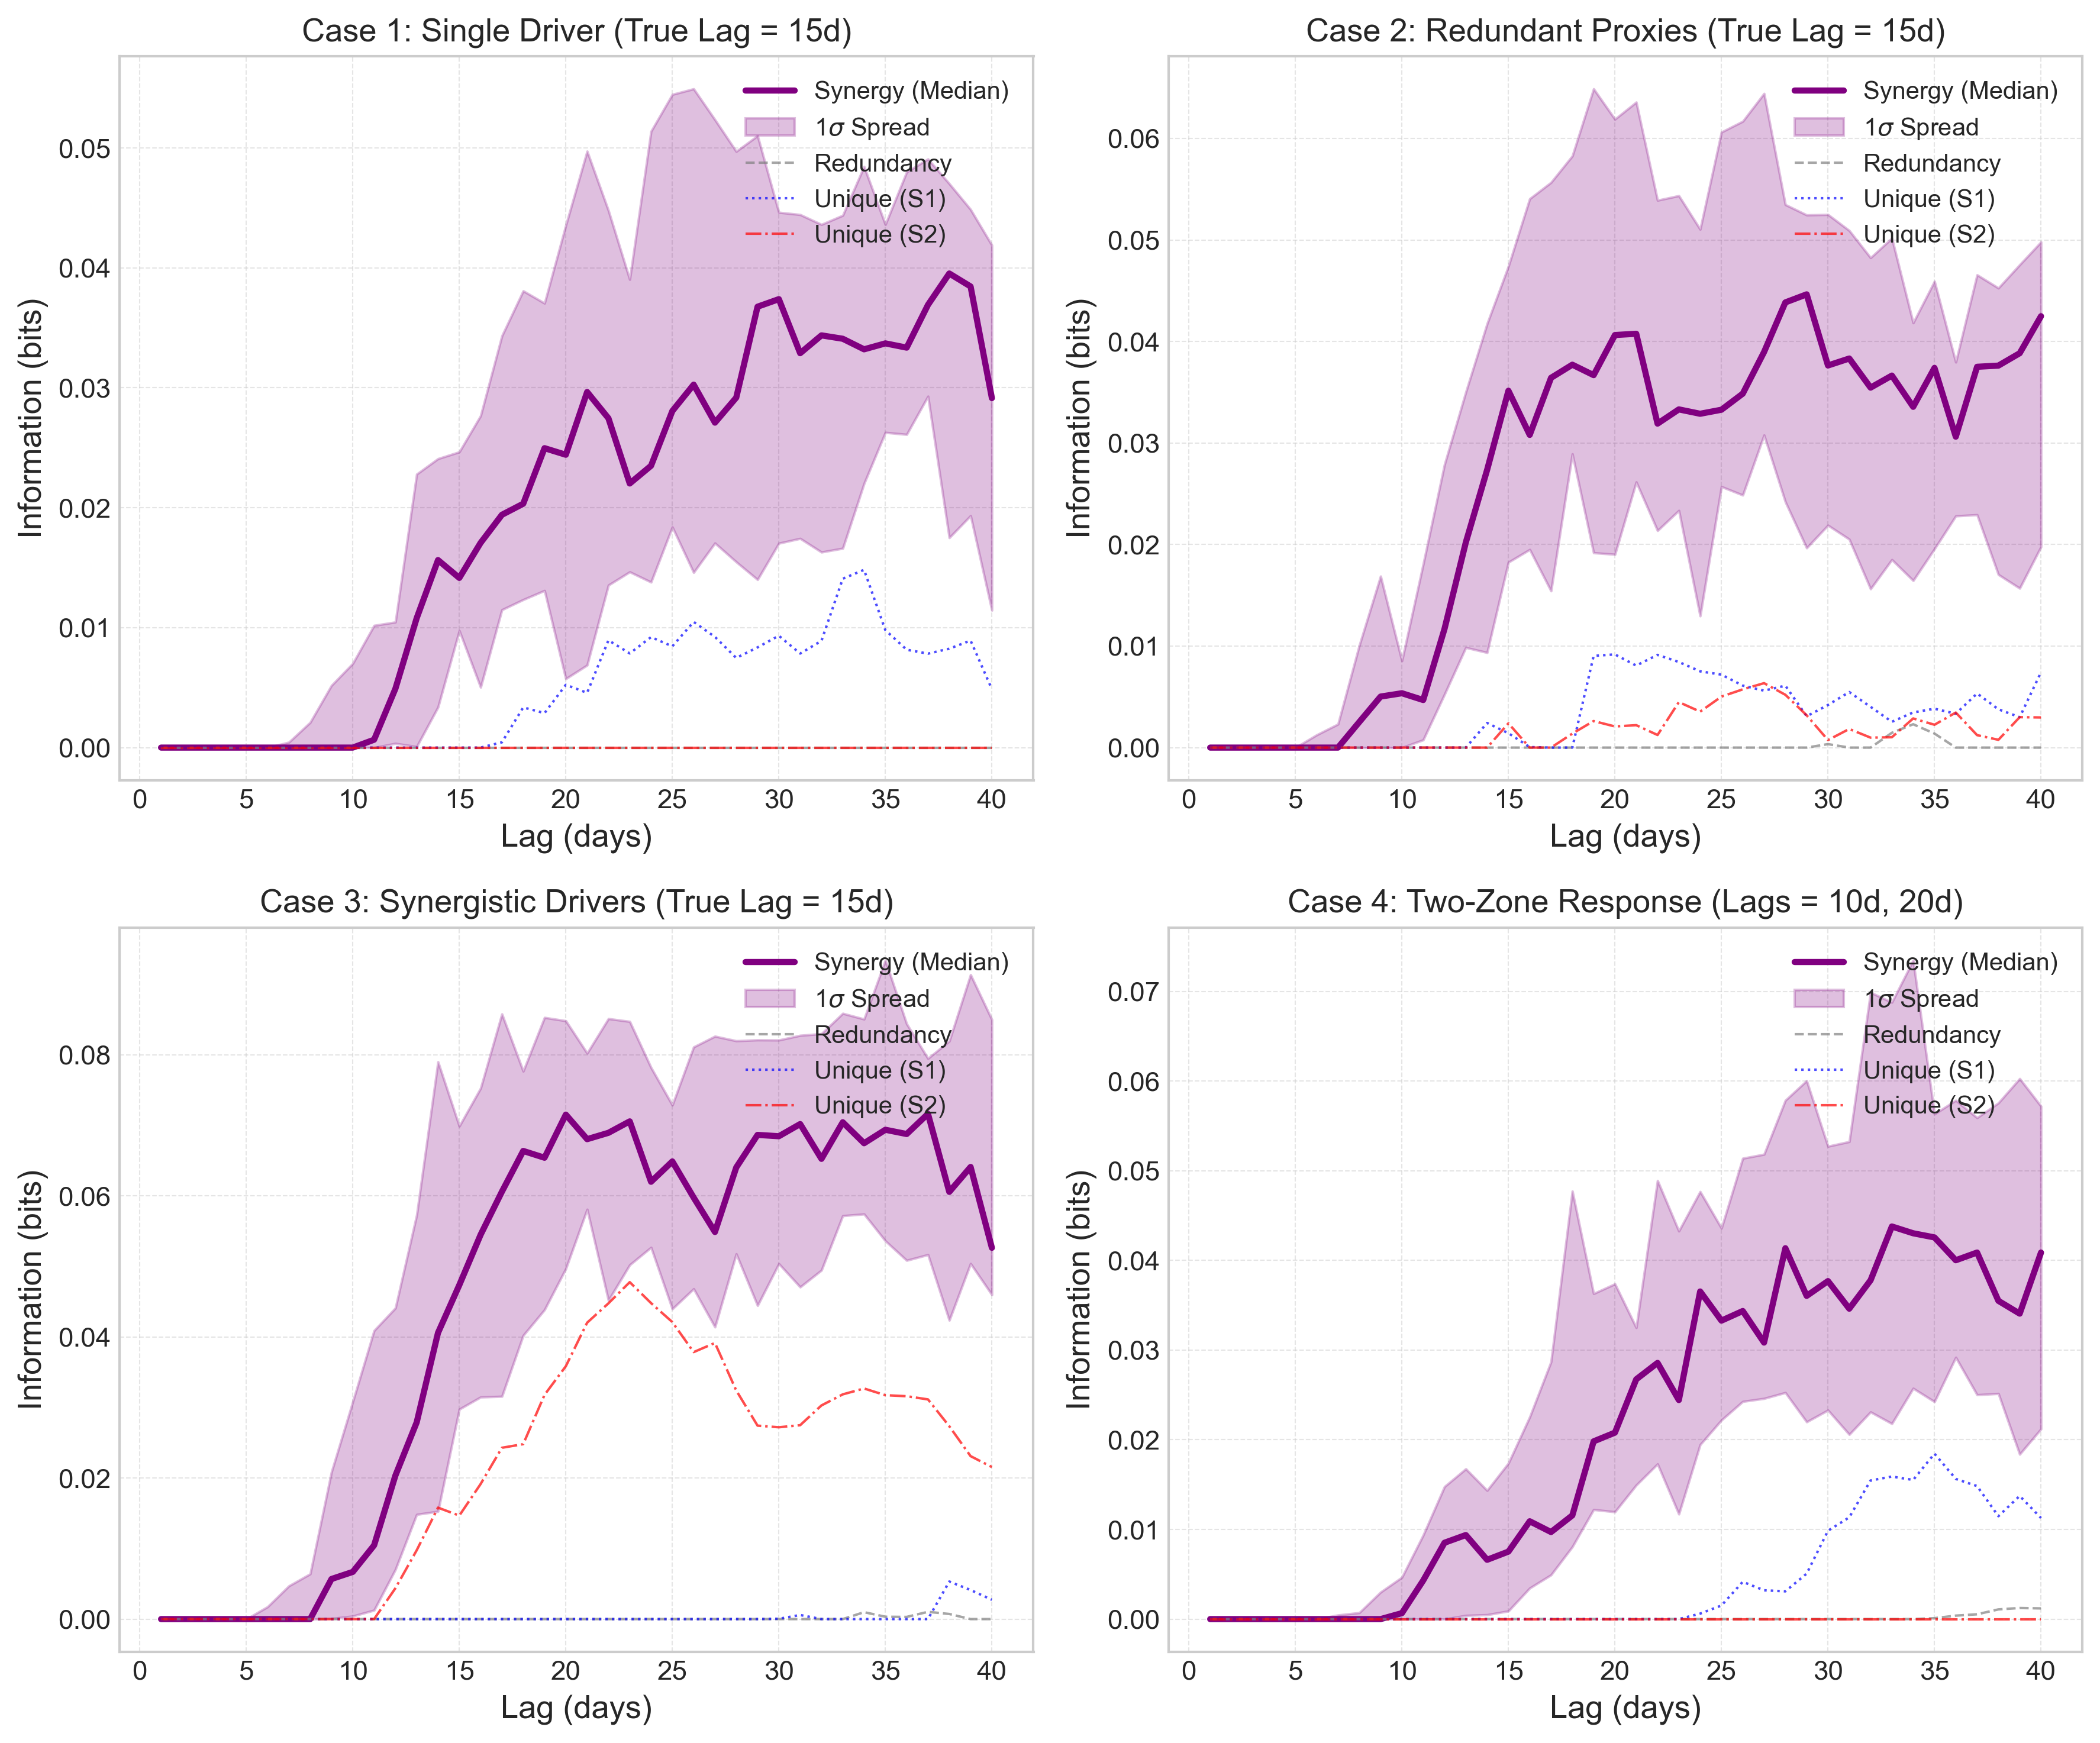
\includegraphics[width=\textwidth]{figure5_synthetic_benchmarks.png}
\caption{SURD information decomposition scans for the four synthetic benchmark cases run under realistic NGC~5548 observational conditions (real sampling, seasonal gaps, and flux errors). Curves represent the Monte Carlo median Synergy (purple, with $1\sigma$ shaded envelope), Redundancy (gray dashed), and Unique information for drivers S1 (blue dotted) and S2 (red dash-dot).}
\label{fig:synthetic_benchmarks}
\end{figure}

\subsection{Target-History Conditioning and Autocorrelation}
\label{sec:target_history_conditioning}

A key challenge in information-theoretic analyses of astronomical time series is distinguishing true cross-component information flow from the target signal's own autocorrelation (red-noise memory). If a target component (such as Core H\(\beta\)) is strongly autocorrelated on short timescales, the apparent synergy between predictors could simply reflect the target's memory rather than causal influence from the driving continuum.

To address this, we perform a target-history conditioned SURD scan. We decompose the conditional mutual information:
\begin{equation}
I(Y(t+\tau); X_1(t), X_2(t) \mid X_3(t))
\end{equation}
where $Y = \mathrm{Core}(t+\tau)$ is the future state of the target Core, $X_1 = \mathrm{Continuum}(t)$ and $X_2 = \mathrm{Blue\ Wing}(t)$ are the predictors, and $X_3 = \mathrm{Core}(t)$ is the target's own past state. This conditional Partial Information Decomposition (conditional PID) is calculated by binning the joint 4D space, extracting the 3D slices for each bin of $X_3$, running the standard SURD decomposition on each slice, and taking the probability-weighted sum of the results.

The results of this comparison are shown in Figure~\ref{fig:history_conditioning}. In the unconditioned case, the synergy curve peaks at a short delay of \textbf{9 days} ($\sim 0.32$ bits), reflecting the strong short-term autocorrelation of the light curve. However, when we explicitly condition out the target's own past, the short-lag synergy is suppressed, and the conditional synergy peak shifts out to \textbf{73 days} ($\sim 0.31$ bits), matching the long-timescale peak found in the main scan. This confirms that the long-term synergy is a genuine cross-component information signature and is not driven by target autocorrelation. Similarly, the unconditioned leak minimum at 1.0 day shifts to 15.0 days in the conditioned case, aligning much more closely with the physical light-travel time of the BLR.

\begin{figure}[ht]
\centering
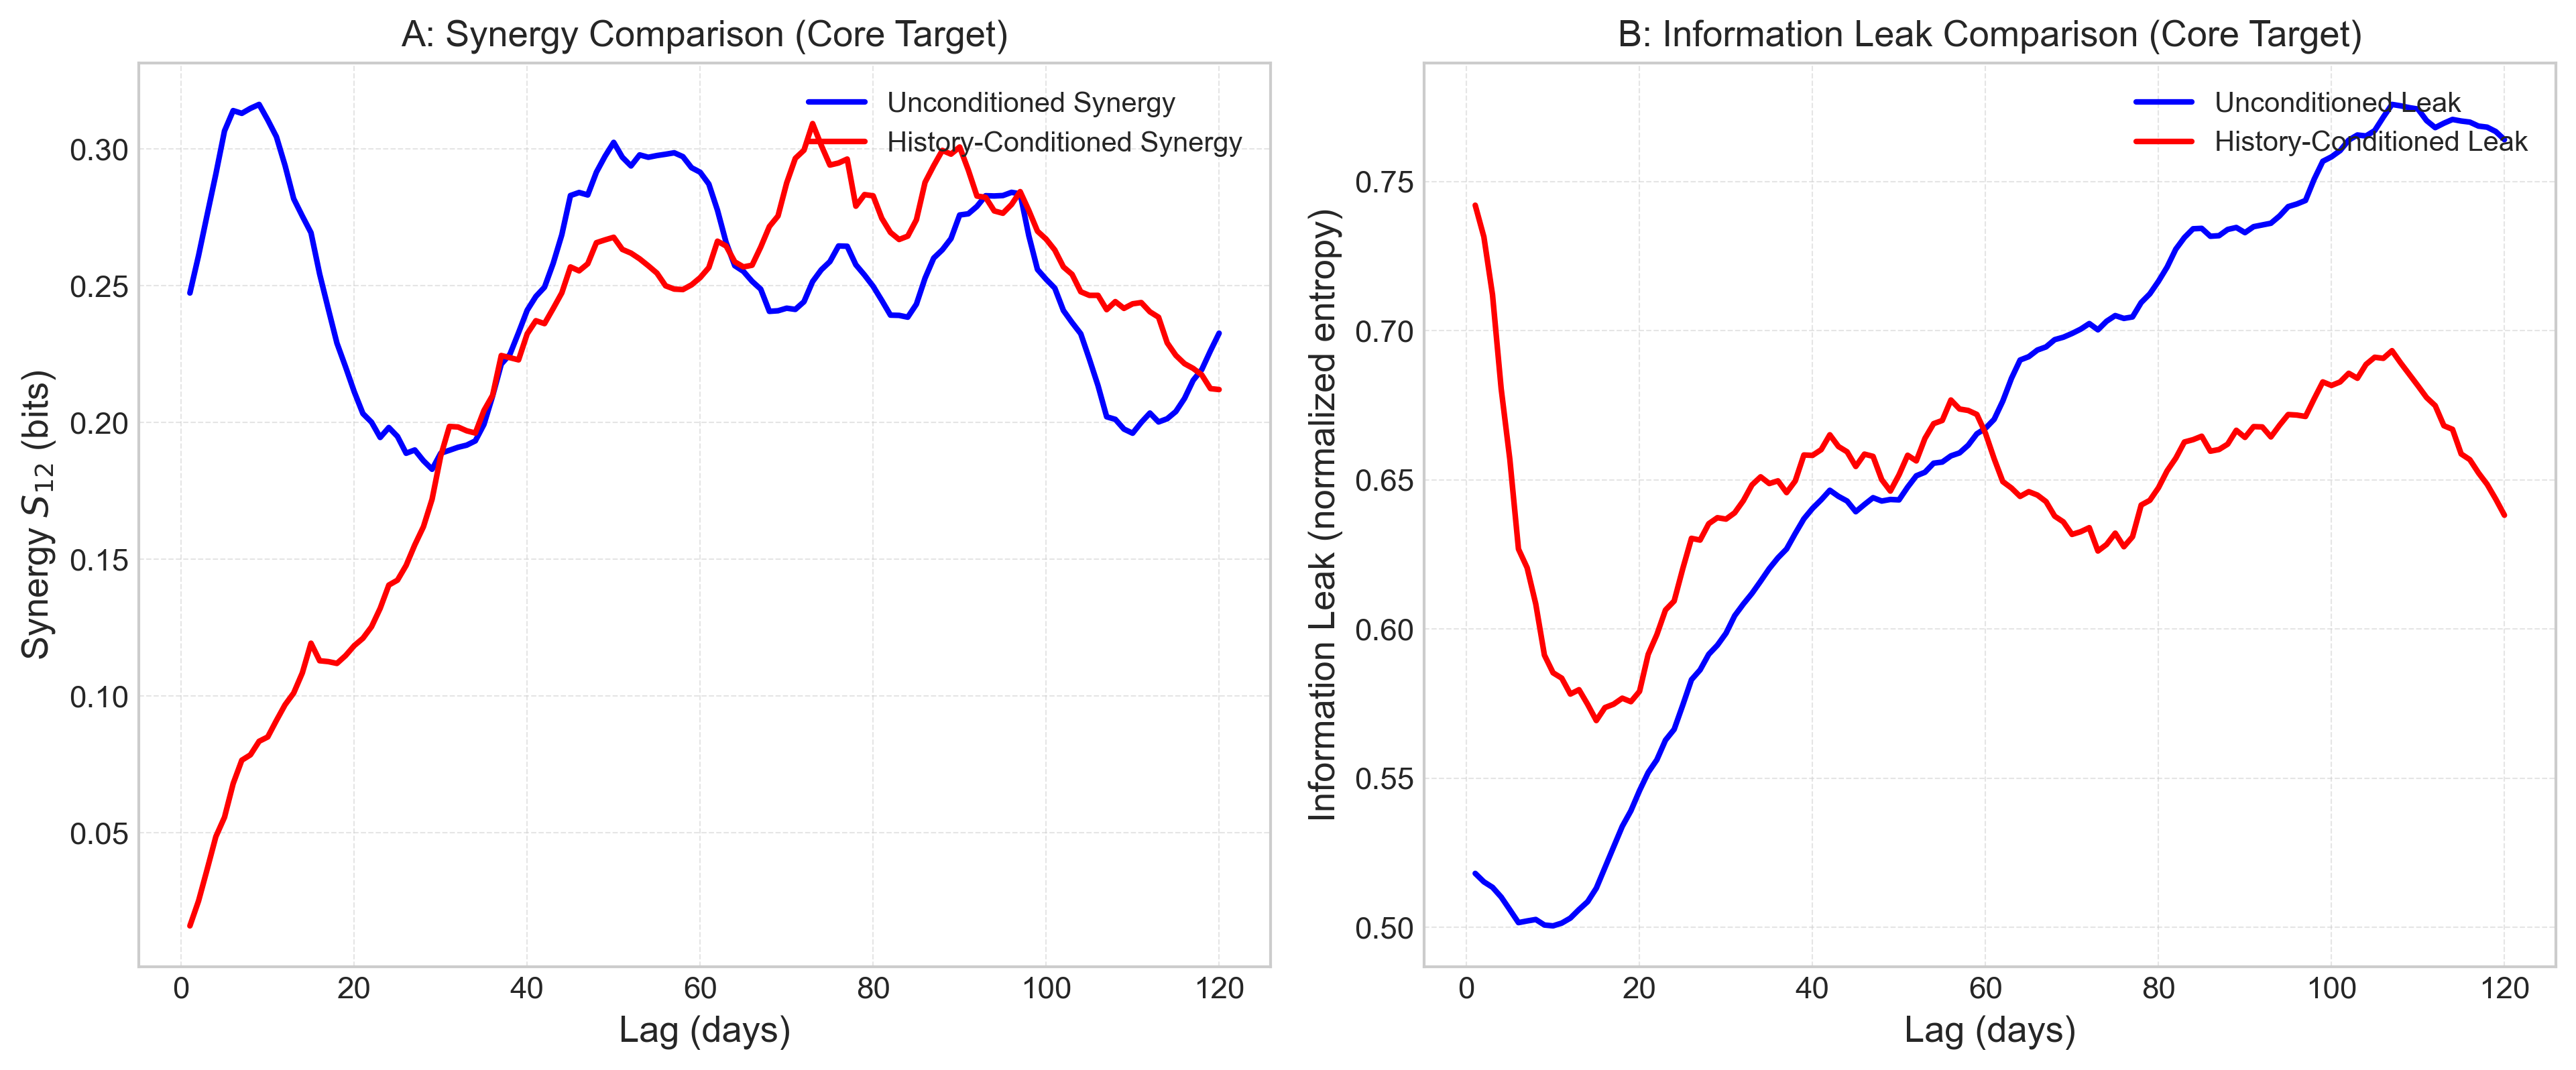
\includegraphics[width=\textwidth]{figure7_history_conditioning.png}
\caption{Comparison of the unconditioned (blue) and target-history conditioned (red) SURD synergy (left) and information leak (right) curves for the Core H\(\beta\) target. Conditioning on the target's own past shifts the synergy peak from a short autocorrelation-dominated delay of 9 days to a robust, long-term cross-component delay of 73 days.}
\label{fig:history_conditioning}
\end{figure}


\section{Astrophysical Interpretation and Discussion}
\label{sec:discussion}

The results in Section~\ref{sec:results} reveal a notable discrepancy between classical linear delays (13--20 days, as measured by both ICCF and JAVELIN) and the SURD synergy peaks (76--119 days). In this section, we discuss the physical implications of these findings for the Broad-Line Region (BLR) of NGC~5548.

\subsection{The Multi-Component Broad-Line Region}

The H\(\beta\) reverberation lag of NGC~5548 is historically reported in the range of 10 to 20 days (e.g., $15.6 \pm 0.5$ days during the high-cadence AGN STORM campaign \cite{Pei2017}). Our ICCF peaks of 13.0 days (Red Wing), 19.0 days (Blue Wing), and 20.0 days (Core), as well as JAVELIN peak delays of $12.8 \pm 1.8$ days (Red), $19.4_{-2.9}^{+2.5}$ days (Blue), and $20.1_{-3.2}^{+2.9}$ days (Core), are in excellent agreement with these standard measurements. They reflect the prompt, linear light-travel response of the broad-line gas to continuum fluctuations.

The fact that the SURD synergy peaks occur at much longer timescales (76 days for the Core, 81 days for the Blue Wing, and 119 days for the Red Wing) suggests that synergy is sensitive to different physical mechanisms or systematic effects than simple linear reprocessing:
\begin{enumerate}
\item \textbf{Extended Geometry:} The long-lag synergy could trace the outer, slow-moving regions of the BLR. In an extended, disk-like or virialized BLR, the outer regions respond with a longer light-travel delay and contribute to the joint information structure of the line profile.
\item \textbf{Non-linear Reprocessing:} While the ICCF measures linear correlation, SURD captures non-linear couplings. The H\(\beta\) emissivity is known to depend non-linearly on the ionizing flux and local gas density, which can manifest as delayed synergistic information that requires both the driving continuum and other line components to resolve.
\item \textbf{Red Noise and Autocorrelation Gaps:} Alternatively, because the long-timescale synergy peaks do not pass global significance tests (FDR), they may arise from systematic properties of the dataset rather than clean physical delays. Specifically, the strong red-noise memory of both the continuum and the line, combined with seasonal observation windows and interpolation across data gaps, can shift unique information into broad synergy envelopes at long lags.
\end{enumerate}

\subsection{Interpretation of the Information Leak}

The normalized information leak, defined as the ratio of conditional entropy to total target entropy:
\begin{equation}
\mathcal{L} = \frac{H(Y(t+\tau) \mid \mathbf{X}(t))}{H(Y(t+\tau))},
\end{equation}
measures the proportion of the target's future uncertainty that remains unexplained by the observed predictors. It is an information-theoretic entropy fraction, not a linear explained-variance statistic (like $R^2$), and it naturally incorporates finite-sample bias, discretization effects, observational noise, missing predictors, and stochasticity.

For all three targets, the unconditioned minimum leak is reached at the shortest lag of 1.0 day, with leak values of approximately $0.085$ for the Core, $0.099$ for the Blue Wing, and $0.151$ for the Red Wing. While this indicates that only $8.5\%$ to $15.1\%$ of the target's entropy remains unresolved, this prompt minimum is driven in large part by the strong autocorrelation (red-noise memory) of the target light curves themselves rather than prompt physical coupling. As shown in Section~\ref{sec:target_history_conditioning}, when we condition out the target's own past state, the conditioned information leak minimum shifts to $\sim 15$ days, which aligns much more closely with the physical light-travel time of the BLR.

As the lag increases beyond these timescales, the information leak rises, representing a loss of predictive power as we move away from the causal horizon. The remaining unexplained entropy (the leak floor) is likely caused by:
\begin{itemize}
\item \textbf{Missing Drivers:} The optical 5100~\AA\ continuum is a proxy for the ionizing extreme ultraviolet (EUV) continuum, which is unobserved. The physical decoupling during events like the ``reverberation holiday'' introduces unexplained variance.
\item \textbf{Measurement Noise:} Observational uncertainties in both the continuum and the spectra limit the theoretical maximum mutual information.
\item \textbf{Discretization and Estimation Bias:} The use of histogram-based probability density estimators with finite binning introduces systematic sample-size bias that prevents the leak from reaching zero.
\end{itemize}

\section{Conclusions and Future Work}
\label{sec:conclusion}

This paper presents the first application of the Synergistic–Unique–Redundant Decomposition (SURD) algorithm to velocity-resolved AGN reverberation mapping data, focusing on the H\(\beta\) profile of NGC~5548. Our main conclusions are:
\begin{enumerate}
\item The V11 Strict Overlap preprocessing pipeline successfully limits edge effects, delivering a reliable, synchronized dataset over the MJD 47512--49255 window.
\item While SURD synergy peaks locally exceed circular-shift and block-bootstrap surrogate envelopes, no individual lag remains globally statistically significant after Benjamini–Hochberg FDR correction. The results indicate a broad information-coupling envelope rather than a mathematically precise physical delay.
\item Classical linear lags (13--20 days, as measured by ICCF and JAVELIN) and SURD synergy peaks (76--119 days) measure fundamentally different mathematical structures. While linear methods track the prompt reverberation response, the long-term synergy profile represents a broad non-linear coupling that remains an area for physical hypothesis testing (such as disk thermal reprocessing, extended geometry, or systematic red-noise effects).
\item The unconditioned minimum information leak at 1.0 day is driven in large part by the strong autocorrelation (red noise memory) of the target light curves. When conditioning out the target's own past history, the leak minimum shifts to $\sim 15$ days, aligning more closely with the physical light-travel time of the broad-line gas.
\end{enumerate}

Future work will focus on applying the SURD framework to larger multi-object databases (such as SDSS-RM or OzDES) to search for population-level trends in synergy and information leakage as a function of black hole mass, luminosity, and accretion rate. Additionally, incorporating X-ray or ultraviolet continuums as joint predictors could help resolve the hidden-driver problem.

\printbibliography


%\bibliographystyle{unsrtnat}
%\bibliography{refs}

\end{document}